%%%%%%%%%%%%%%%%%%%%%%%%%%%%%%%%%%%%%%%%%%%%%%%%%%%%%%%%%%%%%%%%%%%%%%%%%%%%%%%%%
%%                              DISCLAIMER                                     %%
%%%%%%%%%%%%%%%%%%%%%%%%%%%%%%%%%%%%%%%%%%%%%%%%%%%%%%%%%%%%%%%%%%%%%%%%%%%%%%%%%
%% Acest template latex este o propunere bazata pe recomandarile incluse 
%% in ghidul studentului disponibil pe pagina Web a facultatii: 
%% https://ac.tuiasi.ro/studenti/didactic/finalizare-studii/finalizare-studii-calculatoare/finalizare-studii-calculatoare-ghidul-studentului/, 
%% ghid dezvoltat de George Vieriu si adoptat de membrii Departamentului de 
%% Calculatoare al Facultății de Automatică și Calculatoare din Iași cu scopul de 
%% a facilita o redactare corectă și unitară a lucrărilor de diplomă/disertație 
%% ale absolvenților facultății.

%% Va recomandam insistent sa cititi cu atentie ghidul indicat anterior deoarece
%% contine toate informatiile si sfaturile necesare redactarii unei lucrari !!!

%% AVEM RUGAMINTEA CA ORICE EVENTUALA CORECTIE/IMBUNATATIRE sa fie comunicata 
%% si autorilor si review-erilor acestui document, pentru a putea fi ulterior 
%% inclusa intr-o eventuala noua versiune.

%% Autori:
%%      Alexandru Archip: alexandru.archip@academic.tuiasi.ro
%%      Catalin Mironeanu: catalin.mironeanu@academic.tuiasi.ro
%% Review-eri:
%%      Cristian-Mihai Amarandei: cristian-mihai.amarandei@academic.tuiasi.ro
%%      Elena Serban: elena.serban@academic.tuiasi.ro

%% Ideea acestui template a venit ca urmare a unor probleme semnalate de catre
%% studenti in utilizarea LibreOffice in momentul in care era mai mult continut
%% in lucrare si figurile se decalau.

%% In cadrul acestui template au fost folosite atat experienta acumulata, cat si
%% elemente din lucrarile de diploma ale studentilor (in ordine alfabetica):
%%      Valeriu-Mihai Acar (promotia 2021)
%%      Georgiana Atomei (promotia 2021)
%%      Gabriel Cozma (promotia 2021)
%%      George Vrînceanu (promotia 2021)

%% Structura proiect -- elemente importante
%%  1. main.tex - fisierul principal, care va fi compilat
%%              - include lista completa de pachete latex considerate utile
%%              - orice alt pachet considerat necesar va fi inclus tot prin acest fisier
%%  2. Raport1.tex/Raport2.tex - fisierele principale pentru rapoartele intermediare (licenta)
%%  3. pdf      - director in care veti incarca, pentru forma finala, documentele solicitate
%%              (de exemplu: declaratia de asumare a autenticitatii proiectului de diploma, 
%%               semnata si scanata)
%%  4. macros   - director care contine diferite fisiere de configurare
%%              - nu va recomandam sa modificati fisierele:
%%                  configurari.tex, config_anexe.tex, dimensiuni.tex
%%              - actualizati:
%%                  constante.tex: tipul tezei; programul de studiu/specializarea
%%                  student.tex: titlul tezei, numele vostru, gradul si numele coordonatorului
%%  5. coperti  - director care cuprinde copertile externa si interna
%%              - nu ar trebui modificat
%%  6. continut, bibligrafie, anexe
%%              - directoarele care contin o prima propunere de structurare a tezei

%%%%%%%%%%%%%%%%%%%%%%%%%%%%%%%%%%%%%%%%%%%%%%%%%%%%%%%%%%%%%%%%%%%%%%%%%%%%%%%%%
%%                            !! SUCCES !!                                     %%
%%%%%%%%%%%%%%%%%%%%%%%%%%%%%%%%%%%%%%%%%%%%%%%%%%%%%%%%%%%%%%%%%%%%%%%%%%%%%%%%%

%% Template pentru lucrarile de licenta/disertatie/doctorat, bazat pe report ca tip de document
\documentclass[12pt, twoside]{report}

%% limba document
\usepackage[romanian]{babel}
\selectlanguage{romanian}

%% font lucrare
\usepackage[utf8]{inputenc}
\usepackage[T1]{fontenc}
\usepackage{mathptmx}

%% geometria paginii
\usepackage{geometry}
%% setari antet/subsol
\usepackage{fancyhdr}
%% indentare primul paragraf din capitol
\usepackage{indentfirst}
%% cuprinsul include si bibliografia si este navigabil
\usepackage[nottoc]{tocbibind}
\usepackage[unicode, hidelinks, colorlinks, linkcolor=black, urlcolor=blue, citecolor=black]{hyperref}
%% culoare text (pe moment folosit in titluri de capitole)
%% https://www.overleaf.com/learn/latex/Using_colours_in_LaTeX
\usepackage[dvipsnames]{xcolor}
%% format titlu capitol/subcapitol/etc
\usepackage{titlesec}
%% pentru includerea unor pdf-uri externe in document (necesar pentru declaratia de autenticitate)
\usepackage{pdfpages}
%% titluri pentru figuri/tabele/listing-uri de cod/etc.
\usepackage{caption}
%% pozitionare float-uri (figuri/tabele/etc)
\usepackage{float}
%% pentru tabele pe mai multe pagini
\usepackage{longtable}	
%% pentru tabele cu celule cu mai multe linii
\usepackage{multirow}			
%% pentru ecuatii
\usepackage{amsmath}
%% pentru definitii, teoreme
\usepackage{amsthm}
%pentru simboluri de multimi
\usepackage{amsfonts}
%% pentru algoritmi, pachetul algorithm este cel mai basic
\usepackage[chapter]{algorithm}
\usepackage[noend]{algpseudocode}
% daca pachetul algorithm nu este satisfacator pentru ceea ce aveti de scris, mai exista pachetele:
% algorithmic, algorithmicx, algpseudocode, algorithm2e
% https://tex.stackexchange.com/questions/229355/algorithm-algorithmic-algorithmicx-algorithm2e-algpseudocode-confused
%% formatari listing
\usepackage{listings}
% https://www.overleaf.com/learn/latex/Code_listing
%% pachetul minted formateaza/coloreaza sintaxa codului sursa, spre deosebire de pachetul listings care doar face bold pe sintaxa
\usepackage[newfloat]{minted}
% https://www.overleaf.com/learn/latex/Code_Highlighting_with_minted

%% ==================================================================================================== %%
%% pachetele sunt utilizate doar pentru componenta demo
%% TREBUIE SCOASE DIN FORMA DE LUCRU/FINALA
%% pentru text dummy
\usepackage{lipsum}
%% pentru TODO-uri
\usepackage{todonotes}
%% ==================================================================================================== %%

%% pachet pentru parafrazari
\usepackage{quotchap}

%% setup dimensiune pagina, dimensiune header/footer
%% setup dimensiune 16pt
%% valorile generice, pentru documentul in ansamblu
%% in mod uzual, nu ar trebui modificate

%% dimensiune pagina text, header/footer
\geometry{
    a4paper,
    left=2.5cm,
    right=2cm,
    top=2cm,
    bottom=2cm,
    headheight=0.55cm, %% daca am fi mers strict pe 0.5cm, am fi avut warning-uri
    footskip=0.55cm,
}

%% spatiere paragrafe si indentari
\linespread{1.0}                % spatierea intre randuri de 1 rand
\setlength{\parskip}{0pt}       % spatierea intre paragrafe
\setlength{\parindent}{1.27cm}  % identare paragraf de 1.27 cm

%% dimensiune font 16pt
\newcommand{\almostLarge}{\fontsize{16pt}{20pt}\selectfont}
%% date caracteristice universitatii/facultatii.
%% in acest fisier nu trebuie aduse modificari, cu exceptia tipului de teza si a anului in care este sustinuta teza
%% comune: coperta externa si interna
\newcommand{\university}    {UNIVERSITATEA TEHNICĂ „Gheorghe Asachi” din IAȘI}
\newcommand{\faculty}       {FACULTATEA DE AUTOMATICĂ ȘI CALCULATOARE}
\newcommand{\studyfieldlbl} {DOMENIUL: }
\newcommand{\studyfield}    {Calculatoare și Tehnologia Informației}
\newcommand{\studyproglbl}  {SPECIALIZAREA: }
\newcommand{\studyprog}     {Tehnologia Informației}
\newcommand{\promotion}     {2022}
\newcommand{\location}      {Iași}

%% absolventii de master vor inlocui "diploma" cu "disertatie"
\newcommand{\thesistype}    {Lucrare de diplomă}
%\newcommand{\thesistype}    {Lucrare de disertație}
%% datele specifice: nume, prenume student; titlu lucrare; nume, prenume, grad didactic coordonator
%% PENTRU MODIFICARE SE EDITEAZA FISIERUL macros/student.tex
%% date student si lucrare
\newcommand{\thesistitle}   {Analiză comparativă a metodelor clasice și cuantice
de generare a numerelor aleatoare. Aplicație.}    %<---------
\newcommand{\authorlast}    {Stoian}         %<---------
\newcommand{\authorfirst}   {Alin-Bogdan}
\newcommand{\authornamefl}  {\authorfirst \space \authorlast} % first name last
\newcommand{\authornamelf}  {\authorlast \space \authorfirst} % last name first

%% titlul academic si numele coordonatorului stiintific
\newcommand{\coordinator}   {Ș.l. dr. ing. Petrilă Iosif-Iulian}
%% pentru numele complet si grad didactic/titlu academic, consultati https://ac.tuiasi.ro/despre/personal/cadre-didactice-ale-departamentului-de-calculatoare/



\begin{document}

%% elimin header si footer pentru coperti si paginile de cuprins/rezumat
%% \cleardoublepage se inseraza pentru a lasa pagina "verso" libera (pentru versiunile listate
    \pagestyle{empty}
    {
        %% coperta externa
        %% coperta externa
\begin{titlepage}
    \begin{flushleft}
        \Large
        {\university}
        
        \Large
        {\faculty}
        
        \Large
        {\studyfieldlbl \studyfield}
        
        \Large
        {\studyproglbl \studyprog}
    \end{flushleft}
    
    \begin{center}
        % thesis title
        \vspace{7.5cm}
        \Huge
        {\MakeUppercase{\textbf{\thesistype}}}
        
        \vspace{8cm}
    \end{center}

% pentru situatia cu absolvent un pic mai jos    
%    \begin{flushleft}
%        \Large{\bf Coordonator științific:\\}
%        \Large{\textbf{\coordinator}} 
%    \end{flushleft}
    
%    \begin{flushright}
%        \Large{\bf Absolvent:\\}
%        \Large{\textbf{\authornamefl}}
%    \end{flushright}    

% coordonatorul si absolventul pe aceeasi linie    
    \begin{center}
        \begin{minipage}[t]{0.5\textwidth}
    	    \almostLarge{Coordonator științific:}\\
    	    \almostLarge{\coordinator}
        \end{minipage}\hfill
        \begin{minipage}[t]{0.5\textwidth}\raggedleft
    	    \almostLarge{Absolvent:}\\
    	    \almostLarge{\authornamefl}
        \end{minipage}
    \end{center}

    \begin{center}
        % session
        \vfill
        \Large
        \textbf{\location, \promotion}
    \end{center}
\end{titlepage}
        \cleardoublepage
    
        %% coperta interna
        %% coperta externa
\begin{titlepage}
    \begin{flushleft}
        \Large
        {\university}
        
        \Large
        {\faculty}
        
        \Large
        {\studyfieldlbl \studyfield}
        
        \Large
        {\studyproglbl \studyprog}
    \end{flushleft}
    
    \begin{center}
        % thesis title
        \vspace{6.5cm}
        
        \Huge{\textbf{\thesistitle}}
        
        \vspace{1cm}
        
        \Large
        {\MakeUppercase{\thesistype}}
        
        \vspace{7.5cm}
    \end{center}

% pentru situatia cu absolvent un pic mai jos  
%    \begin{flushleft}
%        \large{\bf Coordonator științific:\\}
%        \large{\textbf{\coordinator}} 
%    \end{flushleft}
    
%    \begin{flushright}
%        \large{\bf Absolvent:\\}
%        \large{\textbf{\authornamefl}}
%    \end{flushright}    
    
% coordonatorul si absolventul pe aceeasi linie    
    \begin{center}
        \begin{minipage}[t]{0.5\textwidth}
    	    \almostLarge{Coordonator științific:}\\
    	    \almostLarge{\coordinator}
        \end{minipage}\hfill
        \begin{minipage}[t]{0.5\textwidth}\raggedleft
    	    \almostLarge{Absolvent:}\\
    	    \almostLarge{\authornamefl}
        \end{minipage}
    \end{center}

    \begin{center}
        % session
        \vfill
        \Large
        \textbf{\location, \promotion}
    \end{center}
\end{titlepage}
        \cleardoublepage
    
        %% absolventii de master vor inlocui "declaratie_autenticitate_diploma" cu "declaratie_autenticitate_disertatie"
        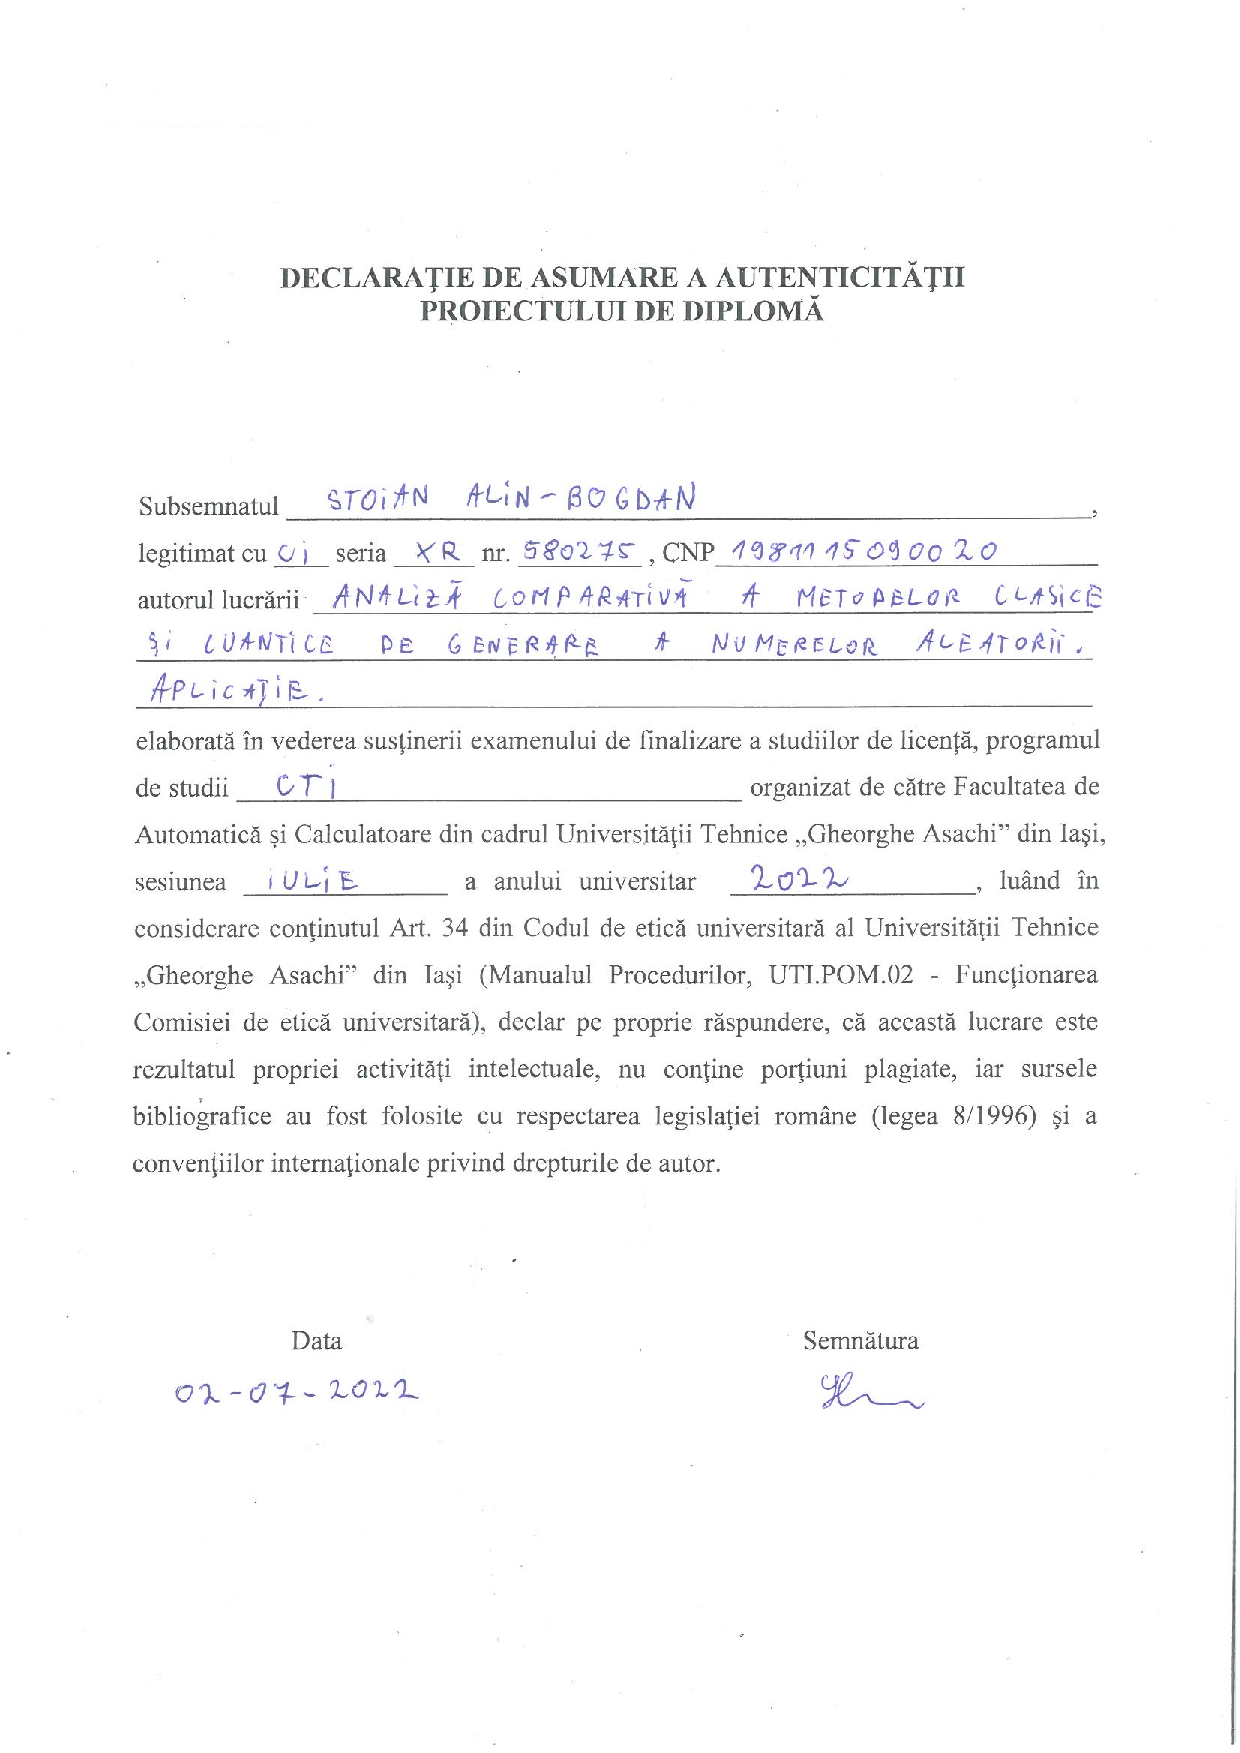
\includepdf[pages=1, scale=1]{pdf/declaratie_autenticitate_diploma}
        \cleardoublepage
        
        %% cuprins
        \renewcommand{\thispagestyle}[1]{}
        \setcounter{tocdepth}{4}
        \setcounter{secnumdepth}{4}
        \tableofcontents
        \cleardoublepage
        
        %%rezumat
        \newpage
\begin{center}
    \LARGE
    \textbf{\thesistitle}
    
    \vspace{0.5cm}
    
    \authornamefl
    
    \vspace{1cm}
    
    \textbf{Rezumat}
    
    \vspace{1cm}
\end{center}


Lucrarea de față își propune topica principală a analizei punctelor tari și a celor slabe a unor eșantioane reprezentative din toate categoriile de generatoare de numere aleatorii, adică propune compararea perfomanțelor și a calității numerelor generate pentru două generatoare de numere pseudoaleatorii (PRNG), un generator de numere aleatorii hardware (HRNG) și mai multe circuite cuantice care duc la generarea de numere aleatorii pe o distribuție uniformă (QRNG).

În acest sens, se prezintă conceptele teoretice ale funcționării QRNG-urilor, formulele de calcul a PRNG-urilor analizate, dar și concepte generale legate de funcționarea generatoarelor de numere aleatorii.

Pe lângă acestea, se prezintă aspecte legate de testele statistice și măsurătorile implementate pentru determinarea calității numerelor aleatorii.

Ulterior, se prezintă cerințele execuției proiectului și bibliotecile / framework-urile utilizate în toate aspectele lucrării, principale printre acestea fiind Qiskit pentru lucrul cu circuite cuantice și PySimpleGUI pentru aplicația cu interfață utilizator.

Apoi, se prezintă pe scurt implementarea PRNG-urilor, a QRNG-urilor și a testelor statistice descrise în primul capitol, apoi și a aplicației cu interfață utilizator. 

În cele din urmă, se prezintă măsurătorile de performanță a generatoarelor, printre care timpii de execuție, dar și parametrii statistici descriși anterior, pe baza cărora se trag niște concluzii. În acest sens, se determină că, în aproximativ toate aspectele în afara aleatorității globale (global randomness), PRNG-urile sunt net superioare.
        \cleardoublepage
    }
    
    %% reset numerotare pagini
    \setcounter{page}{1}
    \pagenumbering{arabic}
    %% import setari generale
    %% creez o comanda nou pentru capitolele ne-numerotate pentru a le putea prelua in header si a le putea adauga la cuprins;
%% in loc de \chapter*{....} va fi \silentchapter{....}
%% sursa de inspiratie pentru \silentchapter{....}: 
%% https://tex.stackexchange.com/questions/89914/chapter-name-in-the-header-with-chapter
\newcommand{\silentchapter}[1]{
    \chapter*{#1}
    \markboth{#1}{#1}
    \addcontentsline{toc}{chapter}{#1}
}

%% notele de subsol vor fi numerotate in continuu pe parcursul tezei
%% fara a mai fi resetate la fieare capitol
\counterwithout{footnote}{chapter}

%% setarile corespunzatoare antetului/subsolului unei pagini de continut
\pagestyle{fancy}
\fancyhf{}
%% pagina impara
%%      antet: titlul capitolului, aliniat in dreapta
%%      subsol: numarul paginii, aliniat in dreapta
\fancyhead[RO]{\nouppercase \leftmark}
\fancyfoot[RO]{\thepage}
%% pagina para
%%      antet: numele autorului, aliniat in stanga
%%      subsol: numarul paginii, aliniat in stanga
\fancyhead[LE]{\authornamefl}
\fancyfoot[LE]{\thepage}

%% setarile corespunzatoare antetului/subsolului unei pagini de inceput de capitol
%% se defineste prin \fancypagestyle{plain}{...}
\fancypagestyle{plain}{
    \fancyhf{}
    \fancyhead[RO]{\nouppercase \leftmark}
    \fancyfoot[RO]{\thepage}
}

%% definitii culori
\definecolor{albastru-ac}{HTML}{004586}

%% Titlu capitol
%% setari format
\titleformat
    {\chapter}%
    [hang]% titlul pe acelasi rand cu eticheta de capitol
    % bold, dimensiune 14pt (pentru normal 12pt), culoare
    {\color{albastru-ac}\bfseries\large}
    {Capitolul \thechapter.\ }% eticheta capitol
    {0pt}% separator
    {}% before-code -- nu setez nimic
    []% after-code -- nu setez nimic
%% setari spatiere
\titlespacing
    {\chapter}%
    {1.27cm}% aliniere la stanga
    {0.42cm}% spatiu inainte de titlul capitolului
    {0.42cm}% spatiu dupa titlul capitolului
    [0pt]% spatiu fata e marginea din dreapta

%% Subcapitol #.# (\section)
%% modul de lucru este acelasi, nu sunt reluate comentariile
\titleformat
    {\section}
    [hang]
    {\color{albastru-ac}\bfseries\itshape}
    {\thesection.\ }
    {0pt}
    {}
    []
\titlespacing
    {\section}%
    {1.27cm}
    {0.42cm}
    {0.21cm}
    [0pt]

%% Subsubcapitol #.#.# (\subsection)
%% modul de lucru este acelasi, nu sunt reluate comentariile
\titleformat
    {\subsection}
    [hang]
    {\color{albastru-ac}\itshape}
    {\thesubsection.\ }
    {0pt}
    {}
    []
\titlespacing
    {\subsection}%
    {1.27cm}
    {0.42cm}
    {0.21cm}
    [0pt]

%% Subsubsubcapitol #.#.#.# (\subsubsection)
%% modul de lucru este acelasi, nu sunt reluate comentariile
\titleformat
    {\subsubsection}
    [hang]
    {\color{albastru-ac}}
    {\thesubsubsection.\ }
    {0pt}
    {}
    []
\titlespacing
    {\subsubsection}%
    {1.27cm}
    {0.42cm}
    {0.21cm}
    [0pt]

%% configurari caption figura
%% - separator .
%% - dimensiune font 11pt (\small)
%% - culoare albastru (similar capitol)
%% - titlul apare centrat sub figura
\captionsetup[figure]{
    labelsep=period,
    font={small, color=albastru-ac},
    justification=centering,
    position=below
}
%% - numerotarea figurilor se face relativ la capitol (George Vieriu style)
\renewcommand{\thefigure}{\arabic{chapter}.\arabic{figure}}

%% configurari caption tabel
%% - separator .
%% - dimensiune font 11pt (\small)
%% - culoare albastru (similar capitol)
%% - titlul apare centrat deasupra figura
%% - namele intrarii de tabel
\captionsetup[table]{
    labelsep=period,
    font={small, color=albastru-ac},
    justification=centering,
    position=above,
    name=Tabelul
}
%% - numerotarea figurilor se face relativ la capitol (George Vieriu style)
\renewcommand{\thetable}{\arabic{chapter}.\arabic{table}}

%% - numerotarea ecuatiilor se face relativ la capitol (non George Vieriu style)
%% (este modul implicit de lucru)
%% - referirea unei ecuatii se face cu comanda \eqref{label:ecuatie}
%% - numerotarea definitiilor si teoremelor nu este precizata in template-ul lui George Vieriu
%% (din nou, am lasat modul implicit de lucru, si anume, relativ la capitol)
\theoremstyle{definition}
\newtheorem{definition}{Definiția}[chapter]
%% - teoreme
\theoremstyle{plain}
\newtheorem{theorem}{Teorema}[chapter]

%% configurari algoritmi
%% - denumire in romana
\floatname{algorithm}{Algoritmul}
%% - este definita o pseudo-instructiunie pentru "eticheta" de pas in proceduri
\makeatletter
\def\BState{\State\hskip-\ALG@thistlm}
\makeatother

%% configurari listing-uri de cod
%% - pachet minted
%% in loc de \begin{listing} {...} \end{listing} va fi folosit noul environment code: \begin{code} {...} \end{code}
%% ceea ce permite ca \begin{minted} {...} \end{minted} sa fie in interiorul \begin{code} {...} \end{code}
\newenvironment{code}{
    \captionsetup{
        type=listing,
        font={small, color=albastru-ac},
        labelsep=period,
        skip=-0.5em, % mut caption-ul putin mai aproape de cod
    }
}{\vspace{1.5em}}

%% - font pentru numarul liniei din cod
\renewcommand{\theFancyVerbLine}{
    \fontfamily{pcr}\small \arabic{FancyVerbLine}
}

%% setarea globala a optiunilor pentru minted, pentru a nu fi scrise de fiecare data dupa \begin{minted}
\setminted{
    frame=none,
    framesep=1mm,
    linenos=true,
    xleftmargin=1em,
    tabsize=2,
    fontfamily=courier,
    autogobble,
    fontsize=\small,
    escapeinside=|| %pentru a putea ava cod latex inside minted (referi linii de cod)
}

%% afisare DOI ca link in bibliografie
% - articolele de jurnal/conferinta pot avea un identificator de tip DOI (Digital Object Identifier)
% - in functie de indexarea articolului, aceasta informatie poate fi:
%       - doi.org - in mod uzual pentru jurnale/conferinte indexate ISI
%       - acm.org - pentru jurnale/conferinte indexate ACM
% - in bibliografie, DOI-ul se trece optional in campul "note", 
%   folosind una dintre cele doua comenzi definite mai jos
\newcommand*{\doi}[1]{DOI: \href{https://doi.org/\detokenize{#1}}{\detokenize{#1}}}
\newcommand*{\doiacm}[1]{DOI: \href{https://dl.acm.org/doi/\detokenize{#1}}{\detokenize{#1}}} 


    
    %% *************** continutul efectiv al lucrarii ***************
    %% dupa fiecare capitol, in main.tex este introdus \cleardoublepage pentru ca fiecare capitol nou sa inceapa pe pagina impara
    \silentchapter{Introducere}
\iffalse
Introducerea va avea 2–3 pagini care vor conține motivația alegerii temei, relevanța și contextul temei alese, obiectivele generale ale lucrării, metodologia și instrumentele utilizate și o scurtă descriere a structurii lucrării (titlul capitolelor, o scurtă descriere și legătura dintre acestea).

În acest capitol nu se introduc figuri, table sau listing-uri de cod. Pot fi în schimb referite!
\fi
\renewcommand{\thesection}{\Roman{section}}
\renewcommand{\thesubsection}{\thesection.\Roman{subsection}}
\section{Motivația alegerii temei}
\subsection{Numerele aleatorii}
Numerele aleatorii, aleatoritatea și generarea de numere aleatorii au aplicații nelimitate într-o mare mulțime de domenii diferite, precum în statistică, criptologie, jocuri, jocuri de noroc, matematică și chiar până și în artă.
Pentru câteva exemple de utilizare a numerelor aleatorii și a metodelor de generare a numerelor aleatorii, aflăm de la Aristotel în "Politica" sa \cite{book:aristotle:2015} că democrația din Grecia antică se baza deseori pe alegeri aleatorii\footnote{"... it is thought to be democratic for the offices to be assigned by lot, for them to be elected is oligarchic." [Aristotle, Politics 4.1294b]}, iar alegerile bazate pe vot puteau fi considerate chiar "oligarhice" în natură. Așadar, numerele aleatorii joacă un rol destul de important în dezvoltarea societății umane, încă de pe vremea celor mai timpurii civilizații!

Până și în ziua de astăzi, unele sisteme politice se bazează pe alegere aleatorii pentru sistemele lor juridice - de exemplu, în sistemul legal anglo-saxon, judecătorii din cadrul unui tribunal sunt deseori aleși aleator pentru a asigura imparțialitate, numerele aleatorii jucând astfel un rol în sistemul legislativ!

Pe lângă aplicațiile din politică, aleatoritatea joacă un rol important până și în sistemele religioase - alegerea unui nou Papă catolic fiind bazată pe culoarea fumului care rezultă în urma arderii unor bilete de vot, pentru a oferi un exemplu din mai multe.

Aplicațiile antice sunt utile pentru a arăta faptul că numerele aleatorii joacă un rol în multiple aspecte ale societății umane din totdeauna, dar probabil că cea mai importantă aplicație a numerelor aleatorii în ziua de astăzi este in contextul criptologiei. O mare parte din metodele de securizare a sistemelor de comunicație în ziua de astăzi sunt bazate pe metode de generare a numerelor aleatorii (de exemplu, în cazul metodelor de autentificare sau în cazul metodelor de asigurare a confidențialității schimbului de date între mai multe sisteme de calcul). A fost dovedit matematic de către Shannon \cite{art:shannon:secrecy:1949} că orice cifru de criptare care asigură proprietatea de "discreție completă" \textit{[en. "perfect secrecy"]} \textbf{trebuie} să îndeplinească aceleași cerințe ca un sistem OTP (One-time pad), care este o tehnică de criptare bazată pe schimbul de o cheie, generată aleator, care nu poate fi mai scurtă decât mesajul trimis, între cele două sisteme de calcul aflate în schimb de mesaje.

Așadar, numerele aleatorii sunt extrem de importante pentru o mare parte din metodele de comunicare moderne (comerț online, sisteme tranzacționale, bancare, naționale, ș.a.m.d), pentru că majoritatea metodelor de creare de securitate sunt bazate, fundamental, pe o componentă aleatorii.

Totuși, dacă "importanța" unui fenomen nu se măsoară în impactul asupra societății, ci în cantitatea de bani generată de existența (sau inexistența) sa, atunci numerele aleatorii, fundamentale pentru industria jocurilor de noroc, sunt cu siguranță unul dintre cele mai importante concepte în existență. În momentul scrierii acestei lucrări, industria globală a cazinourilor și a jocurilor de noroc prezintă o piață în valoare de aproximativ 231 de miliarde de dolari \cite{misc:web:statista:gambling}, cu mult mai mult decât industria fotbalului, de exemplu, care are o valoare de piață de aproximativ 1.9 miliarde de dolari în 2019.

Aș putea să continui aproape la nesfârșit cu aplicațiile numerelor aleatorii într-o cantitate enormă de domenii, atât în trecut, cât și în prezent, dar ideea principală a lucrării de față este faptul de a implementa, a studia și a compara mai multe metode de generare de numere aleatorii, domeniu de studiu important din toate privințele.

\pagebreak

\subsection{Numerele aleatorii "adevărate", pe scurt}
În concepția convențională, există două mari categorii de generatoare de numere aleatorii: generatoare de numere "pseudoaleatorii", numite în continuare PRNG \textit{[en. "Pseudo-random number generator"}, și generatoare de numere aleatorii "adevărate", sau "veritabile", numite în continuare TRNG, sau alternativ HRNG \textit{[en. "True ...", "Hardware..."]}. PRNG-urile sunt simpli algoritmi care se folosesc ori de formule matematice, ori de tabele de numere precalculate pentru a-și produce numerele aleatorii, care par a fi suficient de aleatorii în urma testelor statistice. Domeniul generării numerelor pseudoaleatorii este foarte bine cercetat, iar unele PRNG-uri moderne sunt atât de "bune" încât sunt practic de nedestins cu numerele aleatorii "veritabile". Totuși, problema principală a numerelor pseudoaleatorii este că sunt \textit{deterministe}, adică o secvență de numere poate fi reprodusă, atât timp cât se știe punctul de plecare a acelei secvențe. Totuși, avantajul principal este că sunt \textit{eficiente}, din cauză ca pot produce un număr foarte mare de numere într-un timp foarte scurt. 

Pe de cealaltă parte, numerele aleatorii "veritabile" produse de un TRNG sunt în general extrase dintr-o sursă de \textit{entropie} fizică (voi discuta mai târziu conceptul de "entropie" și TRNG-urile mai în detaliu), sistemele de calcul moderne folosind, de exemplu, informații de la driverele kernel-ului, mișcările mouse-ului, elemente de timing interne sistemului de operare, varianțe din activitatea ventilatoarelor calculatorului, ș.a.m.d. Aceste surse de entropie sunt motivul pentru care acestea sunt uneori numite și "Hardware" Random Number Generators. Diferența principală dintre TRNG-uri și PRNG-uri este faptul că acestea sunt nedeterministe și neperiodice. 

Totuși, pe lângă aceste două categorii, designerii de generatoare de numere aleatorii propun o nouă categorie de generatoare: generatoarele de numere aleatorii \textit{cuantice} \cite{IDQuantique:QuantumvsClassical}. ID Quantique, o firmă elvețiană care produce QRNG-uri \textit{[en. "Quantum ..."]} la nivel hardware, discreditează condițiile fizice meta-stabile sau "haosul" necesar culegerii de entropie în TRNG-uri, și propune generatoarele de numere aleatorii cuantice, bazate pe fenomene cuantice, fundamental probabilistice în acest scop.

Motivația alegerii topicii acestei lucrări este, de fapt, un proiect efectuat în cadrul materiei Sisteme cu Microprocesoare \cite{misc:web:proiectSM}, sub îndrumarea domnului conf. Pantilimonescu, din anul 3 de studii, în cadrul căruia am creat un generator de numere aleatorii "adevărate" utilizând un Raspberry Pi atașat de o cameră web țintită la un ecran cu zgomot alb, utilizând culoarea binară a pixelilor drept sursă de entropie (un pixel alb = '1' logic, un pixel negru '0' logic). În cadrul acelei lucrări, am studiat destul de în detaliu implicațiile numerelor aleatorii în ziua de astăzi, iar această lucrare este un succesor spiritual al aceleia, trecând practic la nivelul cel mai fundamental posibil de 'aleatoritate' pentru un generator de numere aleatorii.

Lucrarea de față își propune analiza "bunătății" celor trei categorii de generatoare de numere aleatorii (conceptul de "bunătate" va fi definit riguros mai ulterior în lucrare), din mai multe perspective, atât prin testarea "aleatorității" secvențelor rezultate, cât și prin testarea empirică a performanței algoritmilor de generare (respectiv, a circuitelor cuantice aplicate în cazul QRNG-urilor). 

\pagebreak

\section{Structura și metodele lucrării}
Lucrarea de față va avea trei mari componente:
\begin{itemize}
    \item Fundamentarea teoretică riguroasă a tuturor conceptelor cu aplicabilitate în interiorul lucrării (ex. fundamentare matematică - matematică complexă și algebră liniară, postulatele mecanicii cuantice, elemente de statistică pentru analiza empirică, etc.). Tot aici vor fi definite specificațiile celor două "aplicații" din cadrul acestei lucrări;
    \item Analiza platformelor pe care se vor executa aplicațiile, motivul alegerii lor, modulele generale și proiectarea în ansamblu a celor două aplicații din lucrare;
    \item Descrierea implementării propriu-zise a aplicațiilor și rezultatele intermediare ale lucrării (în general, statistice).
\end{itemize}

Pe lângă acestea, se va adăuga un capitol de descriere a utilizării celei de-a doua aplicații ("aplicația" propriu-zisă din titlul lucrării), în cadrul căreia se vor prezenta și rezultatele finale ale întregii lucrări și se vor descrie în detaliu rezultatele finale.


În concluzie, lucrarea va încerca a descrie fundamentele necesare înțelegerii conceptelor de generare de numere aleatorii "clasice" și "cuantice" și va prezenta două aplicații, una pentru testarea și prezentarea metodelor utilizate și a doua pentru a oferi o aplicație propriu-zisă, utilizabilă de un end-user, cu interfață grafică ș.a.m.d. Prin contrast, prima aplicație va fi aranjată sub forma unui Jupyter Notebook, prezentând grafic circuitele cuantice utilizate, algoritmii statistici de măsurare a rezultatelor și diverse vizualizări, dar și un script de testare și vizualizare a performanțelor metodelor testate.




\renewcommand{\thesection}{\arabic{section}}
\renewcommand{\thesubsection}{\thesection.\arabic{subsection}}





    \cleardoublepage

    \iffalse

\chapter{Fundamentarea teoretică și documentarea bibliografică}
\label{cap:cap1}

(10–15 pagini)\footnote{Template-ul a fost construit similar celui dezvoltat de George VIERIU, disponibil la \url{https://ac.tuiasi.ro/studenti/didactic/finalizare-studii/finalizare-studii-calculatoare/finalizare-studii-calculatoare-ghidul-studentului/}}

\begin{itemize}
    \item Domeniul și contextul abordării temei;
    \item Tema propusă (formularea exactă a temei, obiective, justificarea abordării);
    \item Prezentare succintă și comparativă privind realizările actuale pe aceeași temă;
    \item Analiza tipurilor de produse/aplicații existente din respectiva categorie a temei,
tehnologii folosite pentru implementare;
    \item Elaborarea specificațiilor privind caracteristicile așteptate de la aplicație. 
\end{itemize}

Lucrările utilizate în dezvoltarea proiectului de diplomă și în redactarea tezei vor fi citate corespunzător în cadrul prezentului document. Această citare trebuie să fie o interpretare sau o descriere proprie autorului prezentei teze asupra ideii/soluției/conceptului prezentat în lucrarea sursă și \textbf{\textit{nu}} o preluare mot-a-mot sau o traducere directă. O posibilă excepție de la această regulă se poate face în cazul rezultatelor teoretice importante, cum ar fi, de exemplu, definițiile, teoremele sau algoritmii suport. În textul asociat citării este recomandat să includeți, de asemenea, și o frază prin care să realizați legătura cu lucrarea proprie. Teza capătă în acest fel consistență și evitați ideea de citare bulk, „doar ca să fie". În continuare vă prezentăm un scurt exemplu.

\todo[inline]{TO DO: Aici ar trebui să introduc o referință bibliografică deoarece ceea ce am scris nu este ideea mea}

Mironeanu et. al. propun o nouă abordare pentru monitorizarea și prevenția atacurilor cibernetice \cite{art:mironeanu:ECAD:2021}. Soluția utilizează tehnici de tip AI/ML și pe un sistem de votare ponderat cu scopul de determina dacă un acces în rețea este un acces normal sau un eventual atac. Pornind de la noțiunile descrise în \cite{art:mironeanu:ECAD:2021}, lucrarea de față își propune îmbunătățirea detecției atacurilor de tip \textit{flood}.

Pornind de la modelul REST propus de Fielding în \cite{thesis:fielding:2000} și considerând specificațiile protocolului HTTP \cite{misc:web:rfc7231}, Archip et. al. demonstrează în \cite{inproc:archip:restful:2018} faptul că o utilizare greșită a modelului amintit poate conduce la o slăbire a securității unui server. Un alt aspect important care trebuie considerat cu privire la securitatea sistemelor informatice este legat de utilizatori. Acest subiect este tratat pe larg în \cite{incollection:ARASEC2020}.

Un exemplu de intrare bibliografică pentru un \textit{tech report} este în \cite[p.~13]{IEEEexample:techreptypeii} (numărul paginii este trecut explicit în sursă). Bineînțeles, nu putem discuta despre configurările și instalările unor sisteme Cloud Computing \cite[p.~113]{book:marinescu:2018}, dacă nu considerăm și sistemele de operare suport sau gazdă \cite{book:operating_systems:2014}. În cazul în care dorim să referim o pagină web care nu se încadrează în categoriile carte, articol, raport tehnic, putem să utilizăm o intrare de tip \verb|misc| în bibliografie. Recomandarea este să utilizăm documente Web publicate de companii importante (precum IBM, RedHat, Apple, etc.) sau personalități recunoscute, precum Bruce Schneier \cite{misc:web:schneier2021}.

\textcolor{gray}{\lipsum}(Figura \ref{fig:puterea_furnizata_pe_cm_cub})

\begin{figure}[H]
    \centering
    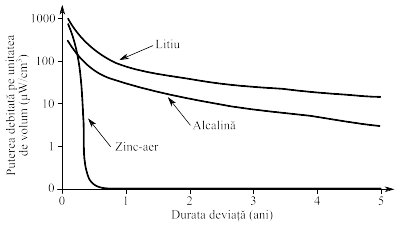
\includegraphics[width=0.6\textwidth]{continut/capitol1/figuri/puterea_furnizata_pe_cm_cub.png}
    \caption{Puterea furnizată pe cm\textsuperscript{3} relativă la durata de viață pentru trei tipuri de baterii.}
    \label{fig:puterea_furnizata_pe_cm_cub}
\end{figure}

\textcolor{gray}{\lipsum}

\section{Exemplu de subcapitol nivel 1}
\label{cap:cap1:ex-subcapitol}

\textcolor{gray}{\lipsum} (Figura \ref{fig:r2_d2})

\begin{figure}[t]
    \centering
    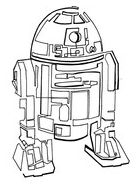
\includegraphics[width=0.25\textwidth]{continut/capitol1/figuri/r2_d2.png}
    \caption{R2-D2\protect\footnotemark}
    \label{fig:r2_d2}
\end{figure}
\footnotetext{imagine preluată de pe un site web care nu „merită” trecut la bibliografie \url{https://www.shutterstock.com/}}

\textcolor{gray}{\lipsum} 

\subsection{Exemplu de subcapitol nivel 2}
\label{cap:cap1:ex-supcapitol:nivel2}

\textcolor{gray}{\lipsum} (Figura \ref{fig:yoda})

\begin{figure}[H]
    \centering
    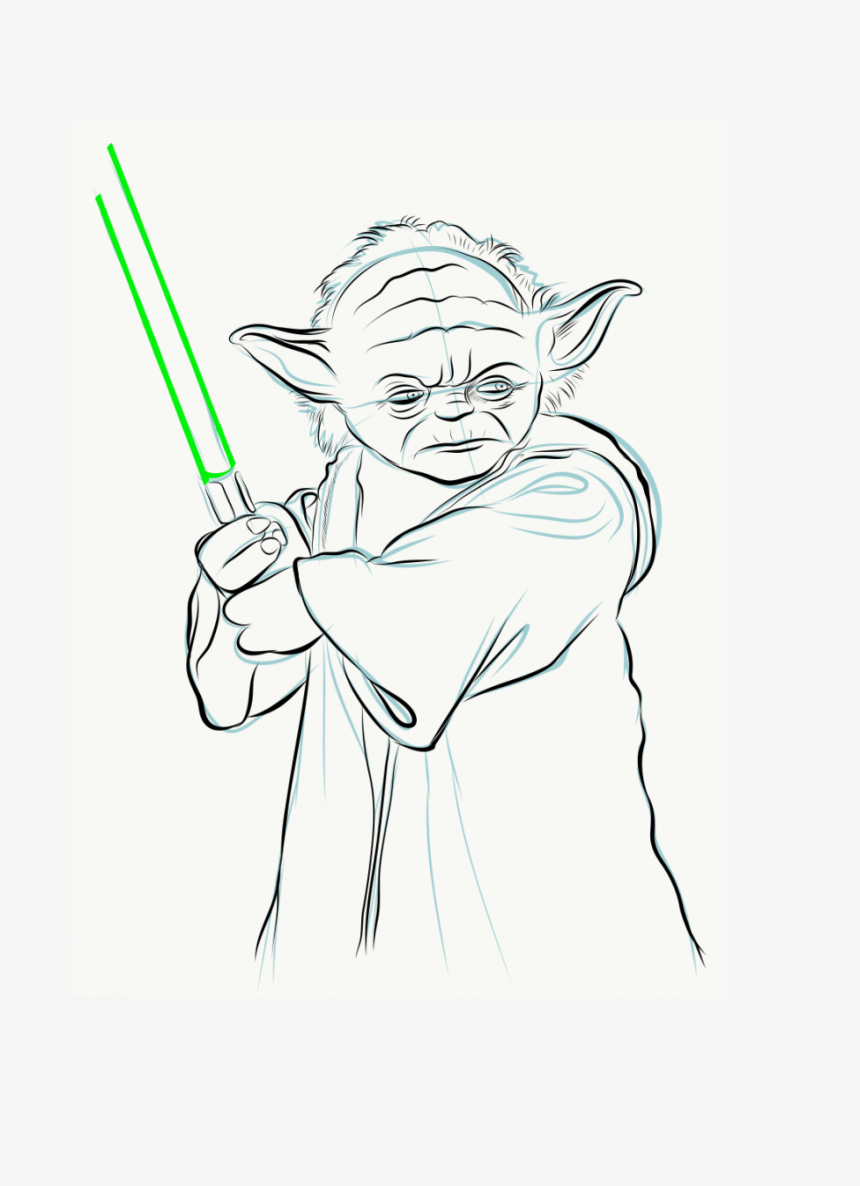
\includegraphics[width=0.3\textwidth]{continut/capitol1/figuri/yoda.png}
    \caption{Yoda\protect\footnotemark}
    \label{fig:yoda}
\end{figure}
\footnotetext{imagine preluată de pe un site web care nu „merită” trecut la bibliografie \url{https://www.pngitem.com/}}

\textcolor{gray}{\lipsum}

\subsubsection{Exemplu de subcapitol nivel 3}
\label{cap:cap1:ex-subcapitol:nivel2:nivel3}

\textcolor{gray}{\lipsum}

Următoarele e fără label FTW, decât să demonstrez gen!\footnote{Dacă vă prindem cu astfel de exprimări, vă scădem 2 puncte!!!}

\section{Nivel 1}
\label{cap:cap1:nivel1}

\subsection{Nivel 2}
\label{cap:cap1:nivel1:nivel2}

Ghilimelele se pun înainte și după reproducerea unui text. Se pun între semnele citării cuvintele sau grupurile de cuvinte citate ironic sau care redau atitudinea rezervată ori dezaprobatoare a autorului față de realitățile pe care le desemnează respectivele cuvinte. Se obișnuiește să se pună între ghilimele titlurile operelor literare de artă sau științifice, ale publicațiilor, numele instituțiilor, firmelor etc. atunci când aceste titluri sunt reproduse într-o frază. 
Atenție: Ghilimelele limbii engleze (“ ”) sunt diferite de ghilimelele limbii române („ ”)!
Observație: Documentele tehnice au adoptat din sintaxa limbajelor de programare ghilimelele duble (") pentru a evidenția șirurile de caractere în text și ghilimelele simple (') pentru evidențierea caracterelor. De exemplu: "acesta este un șir de caractere", acesta este caracterul 'x'.

\subsubsection{Nivel 3}
\label{cap:cap1:nivel1:nivel2:nivel3}

Oricum, mai departe de \verb|#.#.#.#| \textbf{\textit{NU}} trebuie să se ajungă :P.

\fi


\chapter{Fundamentarea teoretică și documentarea bibliografică}
\label{cap:cap1}

Structura următoarelor câteva subcapitole este puternic influențată de structura cursului de Calcul Cuantic din cadrul Facultății de Informatică de la Universitatea "Alexandru Ioan Cuza", predat de doamna Conf. Arusoaie Andreea, fără de care această lucrare probabil că nu ar fi fost posibilă. Voi încerca a prezenta doar elementele relevante, pe scurt, pentru această lucrare, rezumând / scurtând / eliminând acele elemente care nu vor avea nici o legătură cu lucrarea.

\section{Elemente de algebră liniară}

\subsection{Mulțimea numerelor complexe}

Mulțimea numerelor complexe este un sistem de numărare care conține numerele reale și o unitate imaginară $i$ care îndeplinește proprietatea:
\[i^2 = -1\]
Uneori, definiția unității imaginare este dată in literatura de specialitate ca fiind: \[i = \sqrt{-1}\]
Se numește număr complex orice număr de forma \[z = a + ib,\] unde $a$ și $b$ sunt numere reale. Mulțimea numerelor complexe $\mathbb{C}$ este așadar definită în felul următor: 
\[ \mathbb{C} = \{z \enspace|\; z = a + ib,\enspace a,\enspace b \enspace\in\enspace \mathbb{R},\enspace i^2 = -1\} \]

Conjugatul unui număr complex $z$ este definit ca:
\[\bar{z} \overset{not.}{=} z\text{*} = a - ib\]
Notația cu bară deasupra pentru $z$ este deseori utilizată în matematică, iar notația cu asterisc este utilizată mai des în fizică. Pe parcursul acestei lucrări se vor folosi oarecum interschimbabil cele două notații datorită gamei largi de surse de studiu (cărți, cursuri din diferite spații culturale / academice ș.a.m.d.)

Modulul sau amplitudinea unui număr complex:
\[z = \sqrt{a^2 + b^2}\]

\textbf{Proprietăți ale numerelor complexe}:

Fie $z, w \in \mathbb{C}$. Atunci au loc:
\begin{itemize}
    \item $\overline{z + w} = \bar{z} + \bar{w}$ 
    \item $z \cdot \bar{z} = \bar{z} \cdot z = |z|^2$
    \item $\bar{\bar{z}} = z$
    \item $|z| = |\bar{z}|$
\end{itemize}
\pagebreak

Forma trigonometrică a numerelor complexe este dată de formula:
\[z = A(\cos \theta + i \sin \theta) = Ae^{i\theta}\] 

Unde $A = \sqrt{a^2 + b^2}$,  $\theta = \arctan\left(\dfrac{b}{a}\right)$

\subsection{Spații vectoriale}
Fie $V \neq \phi$ și $K$ un corp comutativ peste $\mathbb{R}$ sau $\mathbb{C}$. Un corp este un triplet $(K, +, *)$ în care $K$ este o mulțime cu cel puțin două elemente, iar $+$ și $*$ doi operatori satisfăcând următoarele axiome:
\begin{itemize}
    \item $(K,+)$ este un grup abelian cu un element neutru $0$.
    \item $(K \setminus \{0\}, *)$ este grup cu un element neutru $1$.
    \item Operatorul $*$ este distributiv față de operatorul $+$.
\end{itemize}

Dacă în plus operatorul $*$ este comutativ (adică axioma doi implică conceptul de \textit{grup abelian}), atunci spunem că tripletul $(K, +, *)$ este \textit{corp comutativ}.

Un grup este o mulțime prevăzută cu un operator care combină orice două elemente ale ei pentru a forma un al treilea element în așa fel încât sunt satisfăcute patru condiții, denumite axiomele grupurilor.

Se numește spațiu liniar (sau vectorial) peste K, o mulțime V, inzestrată cu:
\begin{itemize}
    \item \textit{o lege internă} $\enspace+$: \enspace$V \times V \rightarrow V,\enspace (x, y) \rightarrow x + y,\enspace \forall x,y \in V$,
    \item \textit{o lege externă} $\enspace\cdot$: $K \times V \rightarrow V, \enspace (\alpha, x) \rightarrow \alpha \cdot x, \enspace \forall \alpha \in K, x \in V$, 
\end{itemize}

Astfel încât sunt îndeplinite următoarele axiome:

\begin{itemize}
    \item $x + (y + z) = (x + y) + z,  \enspace \forall x,y,z \in V$,
    \item $x + y = y + x, \enspace \forall x, y \in V$,
    \item $\exists0 \in V, \forall x \in V: x + 0 = 0 + x = x$,
    \item $\forall x \in V, \exists (-x) \in V: x + (-x) = (-x) + x = 0$,
    \item $\alpha \cdot (x+y) = \alpha \cdot x + \alpha \cdot y, \forall \alpha \in K, x,y \in V$,
    \item $(\alpha + \beta)\cot x = \alpha \cdot x + \beta \cdot y\ forall \alpha, \beta \in K, x \in V$,
    \item $\alpha \cdot (\beta \cdot x) = (\alpha \beta ) \cdot x, \forall \alpha, \beta \in K, x \in V$,
    \item $1 \cdot x = x, \forall x \in $, unde 1 este elementul unitate din K.
\end{itemize}

Elementele aparținând spațiului liniar $V$ sunt numite vectori, iar elementele aparținând lui $K$ se numesc scalari. Deseori, pentru "legile" interne / externe definite mai sus se folosesc denumirile de "adunarea vectorilor" pentru "+", respectiv "multiplicarea vectorului cu scalar" pentru "$\cdot$". Un element 0 $\in V$ se numește vector nul. În cazul în care $K = \mathbb{R}$, atunci V se numește spațiu liniar real, iar în cazul în care $K = \mathbb{C}$, atunci V se numește spațiu liniar complex. 
Întotdeauna, spațiul stărilor unui sistem cuantic este descris în termenii unui spațiu liniar complex.

În cadrul acestei lucrări, vectorii vor fi considerați a fi în formă \textit{coloană}, adică vor fi scriși în felul următor:
\[
\begin{bmatrix}
1 \\ 2
\end{bmatrix}
\]
dar, de dragul lizibilității vor fi scriși în rând cu textul sub forma (1, 2). În acest caz, se consideră a fi în continuare sub formă coloană.

Fie $\forall n \in \mathbb{N}\text{*}$.

Atunci $\mathbb{C}^n = \mathbb{C} \times \mathbb{C} \times ... \times \mathbb{C}$. Dacă $u \in \mathbb{C}^n, u=(u1, u2, ..., un) \overset{not.}{=} \begin{bmatrix}
u1 \\ u2 \\ ... \\ un
\end{bmatrix}, ui \in \mathbb{C}$.

Atunci, în concluzie, $(\mathbb{C}^n, +, \cdot, \mathbb{C})$ este spațiul vectorial complex adus în discuție anterior, util pentru descrierea spațiului stărilor unui sistem cuantic.

\subsection{Spațiu euclidian complex}

Fie $V$ un spațiu liniar peste $\mathbb{C}$. Se numește produs scalar complex funcția $\braket{\cdot, \cdot}: V \times V \rightarrow \mathbb{C}$ cu proprietățile:
\begin{itemize}
    \item $\braket{u,u} \geq 0, \forall u \in V$,
    \item $\braket{u,u} = 0, \iff u = 0$,
    \item $\braket{u,v} = \overline{\braket{v, u}}, \forall u, v \in V$,
    \item $\braket{u, \alpha v + \alpha ' v '} = \alpha \braket{u, v} + \alpha ' \braket{u ', v}, \forall \alpha, \alpha ' \in \mathbb{C}, u, u ' , v \in V$,
    \item $\braket{\alpha u, v} = \bar{\alpha} \braket{u, v}, \alpha \in \mathbb{C}$.
\end{itemize}

Un spațiu liniar peste $\mathbb{C}$ înzestrat cu produs scalar se numește spațiu euclidian complex sau spațiu prehilbertian.

Produsul scalar a vectorilor $u, v \in \mathbb{C}^n$ este definit prin:
\[
    \braket{u,v} = \sum_{i=0}^{n} \bar{u_i v_i}, \enspace u_i, v_i \in \mathbb{C}
\]
În fizica cuantică, o stare a unui sistem este reprezentată de un vector dintr-un spațiu Hilbert, adică un spațiu vectorial complex dotat cu un produs scalar.

Norma euclidiană a vectorului $u \in \mathbb{C}^n$ este definită prin:
\[
||u|| = \sqrt{\braket{u,u}} = \sqrt{\sum_{i=1}^{n} |u_i|^2}.
\]

\subsection{Baze ortonormale}

Fie $V$ un spațiu euclidian de dimensiune $n$ și fie $B = \{b_1, b_2, ... , b_n\}$ o bază.

$B \subset V$ se numește \textit{bază} a spațiului $V$ dacă $B$ este liniar independentă și Span(B) = V, unde mulțimea Span(U) a unui spațiu euclidian U este definită prin  \[Span(U) =\sum_{i=1}^{n} \alpha_i u_i, \enspace n \in \mathbb{N}\text{*}, u_1, ... u_n \in U\] iar iar elementele $u_1, ..., u_n$ se numesc liniar independente dacă ecuația \[\beta_1 u_1 + ... + \beta_n u_n =0\], are soluție unică$\beta_1 = ... = \beta_n = 0$.


Pentru $\forall u, v \in V$, are loc 
\[
u = \sum_{i=1}^{n} u_i b_i, \enspace v = \sum_{i=1}^n v_i b_i,
\]
iar expresia produsului scalar este 
\[
\braket{u, v} = \sum_{i=1}^{n} \sum_{j=1}^{n} u_i v_j \braket{b_i, b_j}.
\]
Spunem că baza B este \textit{bază ortonormală} dacă
\[
\braket{b_i, b_j} =
\begin{cases}
0, \enspace i \neq j, \\
1, \enspace i = j.
\end{cases}
\]

\subsection{Operatori liniari. Conjugata. Transpusa.}

Fie $\mathcal{L}(X, Y)$ mulțimea operatorilor liniari X cu valori în Y, unde noțiunea de \textit{operator liniar} înseamnă orice aplicație $A: X \rightarrow Y$ unde 
\[
A (\alpha x + \beta y) = \alpha A(x) + \beta A(y), \enspace \forall \alpha, \beta \in \mathbb{C}, \enspace x, y \in X.
\]

Fie $X = \mathbb{C}^m$ și $Y = \mathbb{C}^n$ și fie $A \in \mathcal{L}(X,Y)$.
Operatorul \textit{conjugat} $\bar{A} \in \mathcal{L}(X, Y)$ are matricea asociată definită prin
\[
\bar{A}(i,j) = \overline{A(i,j)}, i \in \{1, ..., m\}, j \in \{1, ..., n\}
\]
Operatorul \textit{transpus} $A^T \in \mathcal{L}(X, Y)$ este operatorul ce are matricea asociată
\[
A^T(i,j) = A(j,i).
\]


\section{Tranziția către calcul cuantic}
\subsection{Notația bra ket (Dirac)}

Voi prezenta puțin mai târziu postulatele mecanicii cuantice, printre care se numără și definiția unui \textit{bit cuantic}, sau \textit{qubit}, dar deocamdată aș dori să prezint notația bra-ket pentru vectori de stare, utilizați intens în următoarele secțiuni. 

Deseori, starea unui qubit este reprezentat de un versor din spațiul de două elemente complexe:
\[
\ket{\psi} = \begin{bmatrix} \alpha \\ \beta \end{bmatrix} \in \mathbb{C}^2,
\]
unde $\alpha, \beta \in \mathbb{C}$. Așadar, $\ket{\cdot}$ - notația \textit{ket} a vectorilor de stare.

Pentru același $\psi$ definit mai sus, definim 
\[
\bra{\psi} = \overline{(\ket{\psi})^T} = \begin{bmatrix}
\bar{\alpha} \bar{\beta}
\end{bmatrix}
\]
Deci, $\bra{\cdot}$ - notația \textit{bra} a vectorilor de stare, care e pur și simplu conjugata transpusă a vectorului de stare scris în notația ket.

\subsection{Produsul scalar pentru spațiul vectorial complex}
Un produs scalar pe un spațiu vectorial complex $V$ este o operație ce asociează fiecărei perechi de vectori $\bra{u}$, $\bra{v}$ un număr complex
\[
\braket{u|v} = \braket{\ket{u}, \ket{v}} = \sum_{i=1}^{n} \bar{u_i}v_i
\]

\subsection{Operatorul adjunct}
Fie $A$ un operator liniar pe un spațiu vectorial $V$. Atunci, există un unic operator $A^\dagger$ pe V astfel încât $\forall \ket{v}, \ket{w} \in V$ să avem
\[
    \braket{v|Aw} = \braket{A^\dagger v | w}.
\]
Operatorul liniar $A\dagger$ se numește operatorul adjunct al lui A (citit deseori și ca "dagger").
În termeni matriceali, $A^\dagger = \overline{A^T}$, unde $\overline{A^T}$ reprezintă conjugata matricei A, transpuse.
Pentru același $\ket{\psi}$ definit în prima subsecție a acestei secții, $\ket{\psi}^\dagger = \bra{\psi} = \overline{\ket{\psi}^T}$.

\subsubsection{Proprietăți ale operatorului adjunct}

Fie $V$ un spațiu Hilbert de dimensiune $n$.
Spunem că operatorul (matricea) A este normal dacă
\[
AA^\dagger = A^\dagger A;
\]
Spunem că operatorul A este hermitian sau autoadjunct dacă 
\[
A = A^\dagger
\]
Spunem că un operator A este \textit{unitar} dacă
\[
A A^\dagger = A^\dagger A = I_n
\]
Operatorii unitari satisfac:
\[
\braket{Au|Av} = \braket{u|v}.
\]

Aceste lucruri vor fi foarte importante când voi prezenta conceptul de \textit{poartă logică cuantică} în următoarele secțiuni.

\subsection{Produsul tensorial}

Fie $U, V$ două spații Hilbert de dimensiune $m$, respectiv $n$. Atunci, produsul tensorial $U \otimes V$ este un spațiu Hilbert, de dimensiune $m \cdot n$.

Pentru doi vectori de stare $\ket{\psi_1} \in U$ și $\ket{\psi_2} \in V$, produsul tensorial este un vector $\ket{\psi_1} \otimes \ket{psi_2}$ din $U \otimes V$.

Dacă A și B sunt doi operatori (matrice) liniari pe $U$, respectiv $V$, atunci $A \otimes B$ este un operator liniar peste $U \otimes V$ definit prin
\[
(A \otimes B) (\ket{\psi_1} \otimes \ket{\psi_2}) \equiv A \ket{\psi_1} \otimes B \ket{\psi_2}
\]

\subsubsection{Reprezentarea matriceală}

Pentru două matrice 
\[
A = \begin{bmatrix}
a_{11} & a_{12} \\
a_{21} & a_{22}
\end{bmatrix}
\]
\[
B = \begin{bmatrix}
b_{11} & b_{12} \\
b_{21} & b_{21}
\end{bmatrix}
\]

Produsul tensorial $A \otimes B$ este definit prin:
\[
A \otimes B = \begin{bmatrix}
a_{11}B & a_{12}B \\
a_{21}B & a_{22}B
\end{bmatrix},
\]
unde $a_{ij}B$ reprezintă înmulțirea matricei B cu un scalar $\implies$ matricea rezultată produsului scalar va fi de dimensiune $4 \times 4$.


\section{Calcul cuantic}

\subsection{Postulatele mecanicii cuantice, din perspectiva calculului cuantic}

În următoarele câteva subsecțiuni voi oferi o perspectivă de ansamblu asupra celor patru postulate ale mecanicii cuantice prezentate de Nielsen și Chuang in \cite{book:QCQI10E:2011}. Voi încerca să combin explicațiile din capitolul 2 a primei părți a cărții cu cele din primul capitol, cu excepția celor despre porți logice cuantice și circuite cuantice, pe care le voi explica după ce termin perspectiva asupra postulatelor mecanicii cuantice, în același fel în care a organizat și doamna Conf. Arusoaie cursul de Quantum Computing menționat anterior.

\subsubsection{\textbf{Postulatul I} - Definiția unui qubit}

Enunțul postulatului este următorul: "Există un spațiu vectorial complex dotat cu produs tensorial (adică, un spațiu Hilbert) asociat oricărui sistem fizic cuantic izolat, cunoscut drept spațiul stărilor a sistemului. Sistemul este descris în totalitate de către vectorul stărilor sale, care este un vector unitar în spațiul stărilor sistemului".

Într-o altă formă, am regăsit enunțul acestui postulat și sub forma următoare: "Oricărei stări fizice posibile a unui sistem cuantic îi corespunde un versor (vector de mărime 1) dintr-un spațiu vectorial complex, dotat cu un produs scalar (spațiu Hilbert)".

Cel mai important lucru este faptul că starea unui sistem fizic cuantic (în cazul ) este descrisă de un versor, numit \textit{vector de stare}. 

Fie $\ket{0}, \ket{1} \in \mathbb{C}$. Atunci definim:

\[
\ket{0} = \begin{bmatrix}
1 \\ 0
\end{bmatrix}
\enspace
\ket{1} = \begin{bmatrix}
0 \\ 1
\end{bmatrix}
\]

Atunci, mulțimea {$\ket{1}, \ket{0}$} este o bază ortonormală a lui $\mathbb{C}^2$. Așadar, orice vector de stare din spațiul stărilor poate fi scris ca o combinație liniară de stări $\ket{0}$ și $\ket{1}$, notat
\[
\ket{\psi} = \alpha\ket{0} + \beta\ket{1},
\]
unde $\alpha$ și $\beta$ sunt numere complexe, uneori numite și "amplitudini cuantice".

În plus, cum starea $\ket{\psi}$ este un versor, satisface proprietatea $||\ket{\psi}|| = 1$, adică
\[
\sqrt{\braket{\psi|\psi}} = 1 \implies |\alpha|^2 + |\beta|^2 = 1.
\]

Așadar, vom numi starea $\ket{\psi}$ drept \textit{bit cuantic}, sau \textit{qubit}.

\subsubsection{Reprezentarea geometrică a qubitului}

Din proprietatea $|\alpha|^2 + |\beta|^2 = 1$ menționată anterior, putem rescrie ecuația sub forma 
\[
\ket{\psi} = e^{i\gamma}(\cos \frac{\theta}{2}\ket{0} + e^{i\varphi}\sin\frac{\theta}{2}\ket{1}),
\]

unde $\theta, \varphi, \gamma$ sunt numere reale. Din cauza unor motive pe care nu le voi detalia aici, factorul $e^{i\gamma}$ din față poate fi eliminat, deoarece nu are nici un efect observabil. Din acest motiv, putem scrie:
\[
\ket{\psi} = \cos \frac{\theta}{2} + e^{i\varphi}\sin \frac{\theta}{2}\ket{1}.
\]

Cum numerele reale $\theta$ și $\varphi$ definesc un punct pe sfera unitate tridimensională, putem folosi o reprezentare numită "sfera Bloch" pentru starea unui bit cuantic. Aceasta este o metodă foarte utilă pentru vizualizarea unui singur bit cuantic, dar din păcate nu există o generalizare trivială a sferei Bloch pentru qubiți multipli. 

\begin{figure}[H]
\centering
    \caption{O sferă Bloch cu un vector $\ket{\psi}$ oarecare și unghiurile $\theta$ și $\varphi$}
    \label{fig:BlochOarecare}
\begin{tikzpicture}


    % Define radius
    \def\r{4}

    % Bloch vector
    \draw (0,0) node[circle,fill,inner sep=1] (orig) {} -- (\r/3,\r/2) node[circle,fill,inner sep=0.7,label=above:$\ket{\psi}$] (a) {};
    \draw[dashed] (orig) -- (\r/3,-\r/5) node (phi) {} -- (a);

    % Sphere
    \draw (orig) circle (\r);
    \draw[dashed] (orig) ellipse (\r{} and \r/3);

    % Axes
    \draw[->] (orig) -- ++(-\r/5,-\r/3) node[below] (x) {$x$};
    \draw[->] (orig) -- ++(\r+0.5,0) node[right] (y) {$y$};
    \draw[->] (orig) -- ++(0,\r+0.5) node[above] (z) {$z$};

    %Angles
    \pic [draw=gray,text=gray,->,"$\phi$"] {angle = x--orig--phi};
    \pic [draw=gray,text=gray,<-,"$\theta$"] {angle = a--orig--z};
    
        
    \draw (0,\r) node[circle,fill,inner sep=2,label={[label distance=0.01cm]75:$\ket{0}$}] (0, 5) {};
    \draw (0,\r) node[circle,fill=white,inner sep=1.5] (0, 5) {};
    
    \draw (0,-\r) node[circle,fill,inner sep=2,label={[label distance=0.01cm]75:$\ket{1}$}] (0, 5) {};
    \draw (0,-\r) node[circle,fill=white,inner sep=1.5] (0, 5) {};


\end{tikzpicture}
\end{figure}

\subsubsection{\textbf{Postulatul II} - Evoluția unui sistem cuantic}

Enunțul postulatului este următorul: "Evoluția unui sistem cuantic închis este descris de o transformare unitară. Așadar, starea $\ket{\psi}$ a sistemului la un moment de timp $t_1$ este legată de starea $\ket{\psi'}$ a sistemului la un moment de timp $t_2$ prin un operator unitar $U$ care depinde \textit{doar} de timpii $t_1$ și $t_2$.

\[
\ket{\psi'} = U\ket{\psi}. 
\]

De observat este faptul că operatorul unitar $U$ (un operator este unitar dacă $U^\dagger U = UU^\dagger = I$) nu poate depinde de $\ket{\psi}$. Acest lucru este important deoarece daca U ar putea depinde de $\ket{\psi}$, calculatoarele cuantice ar putea rezolva cu ușurință probleme NP-complexe, lucru pe care totuși nu îl voi detalia în această lucrare. 

Operatorii unitari $U$ pot fi priviți ca fiind \textit{porți logice cuantice}, dar voi explica circuitele cuantice ceva mai târziu.


\subsubsection{\textbf{Postulatul III} - Măsurarea sistemelor cuantice}

Enunțul este următorul: "Măsurătorile cuantice sunt descrise de o colecție $\{M_m\}$ de operatori de măsurare. Acești operatori se aplică pe spațiul stărilor sistemului măsurat. Indexul $m$ se referă la rezultatele posibile care pot rezulta în urma experimentului. Dacă starea sistemului cuantic este $\ket{\psi}$ în momentul imediat înaintea măsurării, atunci probabilitatea ca rezultatul $m$ să apară este dată de 
\[
p(m) = \bra{\psi}M^\dagger_m M_m \ket{\psi},
\]
iar starea sistemului după măsurare este
\[
\frac{M_m\ket{\psi}}{\sqrt{\bra{\psi}M^\dagger_m M_m \ket{\psi}}}.
\]

Măsurarea unui qubit are două rezultate descrise de doi operatori, $M_0$ și $M_1$, definiți de
\[
M_0 = \ket{0}\bra{0} = \begin{bmatrix}
1 \\ 0
\end{bmatrix} \cdot \ket{0}^\dagger =
\begin{bmatrix}
1 \\ 0
\end{bmatrix}
\cdot
\begin{bmatrix}
1 & 0
\end{bmatrix}
=
\begin{bmatrix}
1 & 0 \\
0 & 0
\end{bmatrix},
\]

\[
M_1 = \ket{1}\bra{1} = \begin{bmatrix}
0 \\ 1
\end{bmatrix} \cdot \ket{0}^\dagger =
\begin{bmatrix}
0 \\ 1
\end{bmatrix}
\cdot
\begin{bmatrix}
0 & 1
\end{bmatrix}
=
\begin{bmatrix}
0 & 0 \\
0 & 1
\end{bmatrix},
\]

\subsubsection{Măsurarea unui qubit în baza computațională}

Dacă presupunem că starea de măsurat este $\ket{\psi} = \alpha\ket{0} + \beta\ket{1}$, atunci probabilitatea de a măsura 0 este dată de 
\[
p(0) = \bra{\psi}M_0^\dagger M_0 \ket{\psi} = \bra{\psi} M_0 \ket{\psi} = |\alpha|^2,
\]
iar probabilitatea de a măsura 1 este
\[
p(1) = \bra{\psi}M_1^\dagger M_1 \ket{\psi} = \bra{\psi} M_1 \ket{\psi} = |\beta|^2.
\]

Faptul că \textbf{probabilitatea}(!!!) de a obține unul dintre cele două numere, 0 și 1 depinde de amplitudinile cuantice $\alpha$ și $\beta$, amplitudini pe care le putem manipula aplicând operatorii unitari descriși anterior este fundamental acestei lucrări. 

Pe lângă măsurarea în baza computațională, adică cu rezultatele așteptate $\ket{0}$ și $\ket{1}$, se poate generaliza postulatul pentru măsuratoarea în orice bază. Acest lucru este foarte important pentru conceptul de entanglement și mulți algoritmi cuantici.

\subsubsection{\textbf{Postulatul IV} - Spații de stare compuse}

Enunț: "Spațiul stărilor unui sistem fizic compus este produsul tensorial al spațiilor stărilor componente".

De exemplu, pentru $n$ sisteme independente, iar sistemul $i$ se găsește în starea $\ket{\psi_i}$, atunci starea sistemului cuantic compus este 
\[
\ket{\psi_{sistem}} = \ket{\psi_1} \otimes \ket{\psi_2} \otimes ... \otimes \ket{\psi_n}.
\]

\subsubsection{Entanglement cuantic, pe scurt}
Spunem că starea $\ket{\psi}$ de 2 qubiți este \textit{entangled} sau "corelată" dacă $\nexists \ket{\psi_1}$ și $\ket{\psi_2}$ astfel încât $\ket{\psi} = \ket{\psi_1} \otimes \ket{\psi_2}.$

Dacă există cele două stări astfel încât să se aplice postulatul 4, se poate spune că starea $\ket{\psi}$ este entangled. De exemplu, starea
\[
\ket{\psi} = \frac{1}{\sqrt{2}}\ket{00} + \frac{1}{\sqrt{2}}\ket{11} 
\] este entangled.

\subsection{Circuite cuantice}

Înainte de a descrie cele câteva porți logice cuantice utile pentru lucrarea de față, aș dori să menționez pe scurt faptul că Deutsch a demonstrat în 1985 \cite{art:Deutsch:QuantumTT:1985} că orice sistem fizic realizabil și finit poate fi simulat perfect cu un model universal de mașină de calcul ce operează cu resurse finite.
Astfel, pentru o mașină Turing clasică care operează cu:
\begin{itemize}
    \item un set finit de stări $S = \{s_1, s_2, ..., s_S, s_{S+1} = {stop}\}$;
    \item un alfabet de simboluri $A = \{a_1, ..., a_A, a_{A+1} = {stop}\}$;
    \item un set finit de instrucțiuni $I = \{i_1, i_2, ... , i_I\}$
\end{itemize}

există un echivalent cuantic, numit \textit{mașină Turing cuantică}, care are spațiul Hilbert al stărilor 
\[
H_T = H_c \otimes H_p \otimes H_m,
\]
unde $H_p$  este spațiul Hilbert al stărilor procesorului, $H_m$ este un spațiu asociat unui număr infinit de qubiți din care se utilizează doar o porțiune finită la un moment dat și $H_c$ este spațiul stărilor asociat cursorului care asigură interacțiunea dintre unitatea de control și banda de memorie.

Așadar, între mașina Turing cuantică și cea clasică există următoarele corespondențe:
\begin{itemize}
    \item $S \rightarrow H_p$,
    \item $A \rightarrow$ spațiul stărilor qubiților $\mathbb{C}^2$,
    \item $I \rightarrow$ evoluțiile unitare în timp a stării cuantice $\ket{\psi} \in H_T$.
\end{itemize}

Mai departe, în această secțiune voi prezenta doar cele câteva porți logice cuantice utile pentru această lucrare, dar voi adăuga și altele într-o anexă, deoarece vor fi utilizate, implicit, în unele metode de generare de numere aleatoare cuantice pe care le voi analiza mai târziu. Atunci când voi utiliza un circuit cuantic a cărui componente sunt generate automat (cu varii porți logice cuantice), voi menționa acest lucru explicit.

Circuitele logice cuantice sunt reprezentate sub forma unor diagrame care arată cam ca în felul următor:
\begin{figure}[H]
    \centering
    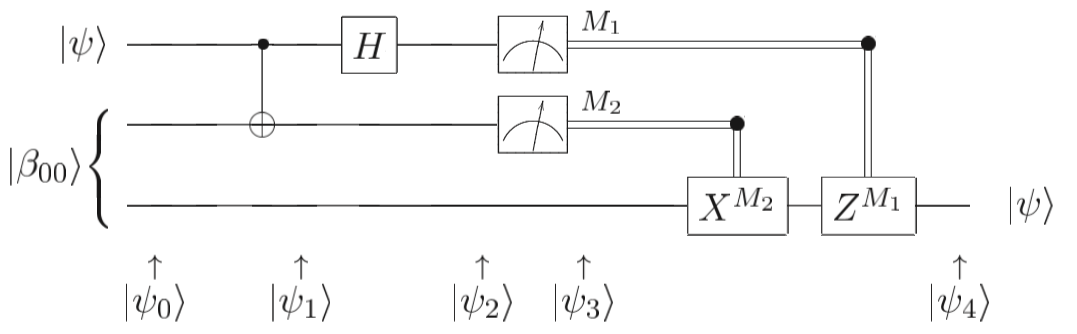
\includegraphics[width=0.6\textwidth]{continut/capitol1/figuri/TeleportationCircuit.png}
    \caption{Circuitul pentru teleportarea unui qubit. Nu voi explica ce înseamnă acest lucru, contează doar cum arată un circuit oarecare.}
    \label{fig:CircuitOarecare}
\end{figure}

Așadar, evoluția sistemului cuantic se interpretează de la stanga spre dreapta; în stânga față de fiecare linie care reprezintă starea fiecărui qubit individual se notează starea inițială a acelui qubit. Deseori, această stare este $\ket{0}$. Porțile logice cuantice pentru qubiți individuali sunt marcați sub forma unui dreptunghi cu un simbol reprezentativ în interior, iar cele care actionează asupra mai multor qubiți sunt reprezentați în diferite feluri, dar fac întotdeauna legătura între liniile mai multor qubiți. Liniile simple sunt pentru qubiți iar liniile duble sunt pentru biți clasici. Simbolul cu un "metru" reprezintă operația de măsurare.

Cea mai și cea mai importantă poartă logică cuantică pentru această lucrare este poarta Hadamard. Poarta Hadamard, față de porțile Pauli (prezentate în anexe), ne permit să ne îndepartăm de polii sferei Bloch și să obținem o superpoziție de $\ket{0}$ și $\ket{1}$. Transformarea Hadamard este definită prin:
\[
H\ket{0} = \frac{1}{\sqrt{2}} \ket{0} + \frac{1}{\sqrt{2}}\ket{1} = \ket{+},
\]
\[
H\ket{1} = \frac{1}{\sqrt{2}} \ket{0} - \frac{1}{\sqrt{2}}\ket{1} = \ket{-}.
\]

Iar reprezentarea matriceală a transformării Hadamard este 
\[
H = \frac{1}{\sqrt{2}}\begin{bmatrix}
1 & 1 \\
1 & -1
\end{bmatrix}
\]

De asemenea, transfomarea Hadamard poate fi exprimată ca o rotație de 90 grade în jurul axei Y, urmată de o rotație de 180 grade în jurul axei X, notat
\[
H = XY^{1/2},
\]
unde X și Y sunt porțile Pauli, notația cu exponent $\frac{1}{2}$ reprezentând o jumătate de rotație.

Efectul porții Hadamard:
\begin{figure}[!htb]
\minipage{0.5\textwidth}
  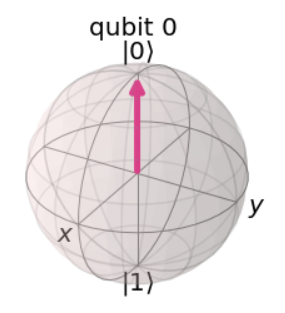
\includegraphics[width=\linewidth]{continut/capitol1/figuri/BlochDefault.png}
  \caption{Starea unui qubit inițializat în $\ket{0}$}\label{fig:bloch_default1}
\endminipage\hfill
\minipage{0.5\textwidth}
  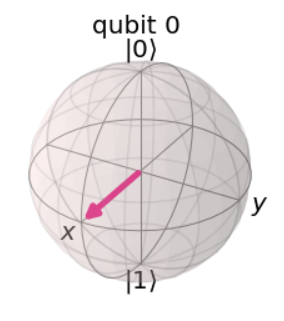
\includegraphics[width=\linewidth]{continut/capitol1/figuri/BlochHadamard.png}
  \caption{După aplicarea transformării Hadamard}\label{fig:bloch_hadamard}
\endminipage\hfill
\end{figure}

Așadar, cum amplitudinile cuantice $\alpha$ și $\beta$ din definiția qubitului sunt, după aplicarea porții Hadamard, amândouă $\frac{1}{\sqrt{2}}$, probabilitatea de obține fiecare dintre cele două stări, $\ket{0}, \ket{1}$ după măsurare este $(\frac{1}{\sqrt{2}})^2$, adică exact 1/2! Acest lucru practic trivializează conceptul fundamental a lucrării de față, adică acela de a realiza un generator de numere aleatoare folosind calculul cuantic, deoarece o simplă aplicare a porții Hadamard obține generarea unui număr cuantic exact uniform! Totuși, în capitolele următoare, voi realiza mai multe metode de generare a numerelor aleatoare cuantice și voi încerca să le demonstrez corectitudinea (adică, numerele generate sunt cu adevărat aleatoare) și să le măsor performanțele. În acest scop, pe lângă poarta Hadamard voi mai folosi următoarele porți:

\begin{itemize}
    \item Poarta de rotație generică în jurul axei y Ry
\end{itemize}
Ry este o poartă de rotație parametrizată. Reprezintă o rotație de $\theta$ radiani în jurul axei y. Trasformatea Ry este următoarea:
\[
R_y(\theta) = \begin{bmatrix}
\cos \frac{\theta}{2} & -\sin \frac{\theta}{2} \\
\sin \frac{\theta}{2} & \cos \frac{\theta}{2}
\end{bmatrix}
\]

În acest sens, pentru $\theta = \frac{\pi}{2}$, efectul acestei porți este exact același cu cel a unei porți Hadamard pentru un qubit inițializat în starea $\ket{0}$, fără "overhead"-ul unei rotații suplimentare în jurul axei x, lucru care, cum voi observa în capitolele următoare, are un efect relevant asupra performanței unui calculator cuantic!

\begin{itemize}
    \item Poarta de rotație generică U3
\end{itemize}

Aceasta este o poartă logică parametrizată care reprezintă o rotație cu 3 unghiuri Euler. Nu am găsit multă documentație despre aceasta, dar aceasta este deseori descompusă de fapt în câteva alte rotații:

\[
U3(\theta, \phi, \lambda) = RZ(\phi)RX(\phi/2)RZ(\theta)RX(\pi/2)RZ(\lambda),
\]
Unde $RX, RZ$ reprezintă porți generice de rotație în jurul axelor X, respectiv Z, similar cu poarta Ry descrisă anterior. De observat fapul că poarta U3 nu se folosește de o poartă Ry în descompunerea ei, motiv pentru care am analizat și performanța ei pentru generarea numerelor aleatoare. Reprezentarea matriceală a porții este următoarea:
\[
U3(\theta, \phi, \lambda) = \begin{bmatrix}
\cos\frac{\theta}{2} && -e^{i\lambda} \sin \frac{\theta}{2} \\
e^{i\phi}\sin \frac{\theta}{2} && e^{i(\phi + \lambda)} \cos \frac{\theta}{2}
\end{bmatrix}
\]

\section{Teste statistice}

Cum o mare parte din această lucrare se axează pe măsurarea performanțelor și corectitudinii mai multor metode de generare de numere aleatoare, mă voi utiliza de mai multe teste statistice pentru a verifica distribuțiile numerelor rezultate (voi testa uniformitatea numerelor generate în cazul scopului generării unei distribuții uniforme și normalitatea în cazul generării unei distribuții normale). Dar, înainte de a prezenta testele statistice, voi discuta câteva elemente de bază de statistică.

\subsection{Testarea ipotezelor statistice}

Formularea corectă de ipoteze statistice este probabil cel mai important aspect al cercetării din punct de vedere statistic. În acest sens, testarea statistică se face prin enunțarea a două ipoteze și apoi acceptarea (sau respingerea) ipotezei nulului:
\begin{itemize}
    \item Ipoteza nulului ($H_0$): reprezintă modelul pe care se dorește a se înlocui (respinge)
    \item Ipoteza alternativă ($H_1$): noul model, care în majoritatea cazurilor reprezintă negația ipotezei nulului.
\end{itemize}

Prin respingerea ipotezei nulului, se afirmă faptul că rezultatele nu sunt datorate întamplării și se poate spune că rezultatul obținut este seminificativ din punct de vedere statistic.

\subsection{Pașii unui test statistic}
\begin{itemize}
    \item Formularea problemei în termenii ipotezelor statistice,
    \item Alegerea unui test statistic și o metrică asociată potrivită pentru problemă
    \item Alegerea unui nivel de semnificație și apoi calcularea pragului de separare (valoarea critică) dintre valorile acceptabile și cele considerate inacceptabile (de obicei, o probabilitate de 95 sau 99\%),
    \item Calcularea parametrilor statistici folosind datele eșantionului
    \item Compararea valorii calculate cu valoarea critică pentru a decide dacă ipoteza nulului se respinge sau se acceptă.
\end{itemize}

\subsection{Valoarea p}

În statistică, valoarea p este probabilitatea obținerii de rezultate cel puțin la fel de extreme ca rezultatele observate ale unui test statistic, asumând că ipoteza nulului este corectă. Valoarea p, care inseamnă valoare a probabilității, este un instrument statistic de masură, cu valori cuprinse între 0 și 1. Este folosită în cadrul testării ipotetice. 

Valoarea p se calculeaza pornind de la deviația dintre o valoare observată și o valoare aleasă de referință, știind funcția densitate de probabilitate a statisticii, cu o diferență mai mare însemnând o valoare mai mică pentru valoarea p. 

Deci, valoarea p reprezintă probabilitatea ca efectele observate să fie la fel de mari ca cele din studiu. Dacă valoarea p este mică, rezultatele studiului nu se datorează intâmplării și respingem ideea că nu există nicio diferență între cele doua eșantionane (respingem ipoteza nulului). Dacă valoarea p este mare, diferențele observate se datorează cel mai probabil intâmplării și nu vom respinge ideea că nu există diferențe între eșantioane.

Valoarea p va fi utilizată deseori în această lucrare pentru a verifica corectitudinea respingerii ipotezelor enunțate de către mine.

\subsection{Testul Z pentru compararea mediilor a două eșantioane cu varianțe inegale}

Parametrul testului este
\[
z = \frac{\bar{X}_1 - \bar{X}_2}{\sqrt{\frac{s_1^2}{n_1} + \frac{s_2^2}{n_2}}},
\]
unde
\begin{itemize}
    \item $\bar{X_1}$ = media primului eșantion,
    \item $n_1$ = volumul primului eșantion,
    \item $s_1^2$ = varianța primului eșantion.
\end{itemize}
Idem pentru al doilea eșantion.
Comparând acest z calculat cu valoarea z dintr-un tabel al valorii z normale, se determină în acest fel regiunea critică a testului (bilateral sau unilateral) și se acceptă sau respinge ipoteza nulului în funcție semnul de comparare dintre valoarea calculată și cea din tabel.

\subsection{Testul Kologomorov-Smirnov}

Este un test neparametric pentru testarea egalității a două funcții de distribuție care poate fi utilizat pentru a compara un eșantion cu funcție de distribuție de referință sau a compara două eșantioane a căror distribuție nu se cunoaște. În acest sens, mă voi folosi de acest test pentru a compara rezultatul unei generări de numere aleatoare care să urmeze o distribuție normală (de exemplu, functia $randn()$ din Matlab cu o distribuție normală cu aceeași parametri ca cei utilizați de distribuția dorită.

Din păcate, documentația pentru acest test este cam slabă, și nu prea am reușit să găsesc o metodă implementă în vreun limbaj de programare, așa că acest test este singurul pentru care mă voi folosi de o implementare nefăcută de mine. Singurul motiv pentru care fac acest lucru este deoarece sunt absolut sigur că acest test este cel mai potrivit pentru cerințele mele.

Parametrul testului pentru o funcție cumulativă de distribuție $F(x)$ este
\[
D_n = \sup_x |F_n(x) - F(x)|,
\]
unde $\sup_x$ este supremum-ul setului de distanțe. Intuitiv, statistica ia cea mai mare diferență în modul a celor două funcții de distribuție pentru toate valorile $x$.



    \cleardoublepage

    \iffalse
\chapter{Proiectarea aplicației}
\label{cap:cap2}

(10–20 pagini)

\begin{itemize}
    \item se analizează platforma hardware pe care va fi executată respectiva aplicație și se analizează care abordare în implementare ar fi mai bună pentru respectiva structură
    \item se stabilesc modulele generale ale aplicației și interacțiunile dintre ele;
    \item se analizează avantaje și dezavantajele metodei alese;
    \item se indică limitele în care metoda va funcționa. 
\end{itemize}

\textit{Componente software:}
\begin{itemize}
    \item proiectarea propriu zisă (diagrame ER pentru baze de date, UML pentru proiectele care necesită diverse paradigme complexe și lucru cu clase – orientat obiect, scheme logice pentru cei care dezvoltă în limbaje structurate etc);
    \item se stabilește tehnologia aleasă pentru implementare și se justifică alegerea făcută;
    \item se descriu succint numai clasele dezvoltate și implementate de absolvent cu trimitere la pagina din anexă unde se află codul complet;
\end{itemize}

Figurile mai complexe, care nu se văd bine în format A4/portrait, pot fi incluse în anexe și referite normal (vezi Figura \ref{fig:AT} din Anexa \ref{anexa3:func_xyz}).

\vspace{1em}

\textit{Componente hardware:}
\begin{itemize}
    \item stabilirea componentelor hardware necesare. Exemplu: etaje analogice, display-uri, dispozitive I/O, periferice USB, etc.;
    \item analiza performanțelor și descrierea perifericelor procesorului/microcontrolerului folosit
    \item realizarea schemei bloc care să reflecte interconectarea componentelor principale;
    \item simularea funcționării componentelor hardware (OrCAD, Proteus, simulatoare HDL);
    \item proiectarea cablajului imprimat (Altium Designer, Eagle).
\end{itemize}

\textcolor{gray}{\lipsum} (Figura \ref{fig:BB8})

\begin{figure}[H]
    \centering
    
\includegraphics[width=0.3\textwidth]{continut/capitol2/figuri/BB8.png}
    \caption{BB8\protect\footnotemark}
    \label{fig:BB8}
\end{figure}
\footnotetext{imagine preluată de pe un site web care nu „merită” trecut la bibliografie \url{https://www.pngitem.com/}}

\textcolor{gray}{\lipsum}

Ecuația \eqref{eq:sample} este un exemplu foarte simplu de formulă matematică. Ecuațiile vor fi referite prin comanda \LaTeX\ \verb|\eqref{}| din pachetul \verb|amsmath|.

\begin{equation}
    \label{eq:sample}
    e^{\pi i} + 1 = 0
\end{equation}

\begin{equation}
    \label{eq:multiline_sample}
    \begin{split}
        A & = \frac{\pi r^2}{2} \\
         & = \frac{1}{2} \pi r^2
    \end{split}
\end{equation}

În ecuația \eqref{eq:multiline_sample} avem un prim exemplu multiline.

Ecuațiile, definițiile și teoremele se referă în textul lucrării de licență/disertație prefixate: ecuația \eqref{eq:sample}, definiția \ref{def:diploma} sau teorema \ref{thm:equal}, iar aici este o pură întâmplare că au același indice, fiind vorba despre prima ecuație, prima definiție și prima teoremă din Capitolul \ref{cap:cap2}.

În continuare, definiția \ref{def:diploma} introduce conceptul de „Lucrare de diplomă”. Titlul efectiv este opțional și îl regăsiți în \LaTeX\ între [].

\begin{definition}[Lucrare de diplomă]
    \label{def:diploma}
    Lucrarea de diplomă face dovada nivelului și calității pregătirii profesionale, teoretice și aplicative a absolventului, iar prin modul în care aceasta este prezentată (susținută public în fața unei comisii de examinare) ea evidențiază calitățile științifice și inginerești definitorii ale absolventului.
\end{definition}

Numerotarea teoremelor se va face similar ecuațiilor și definițiilor de mai sus. Vezi teorema \ref{thm:equal}.

\begin{theorem}[Teorema egalității]
    \label{thm:equal}
    Dacă $a=b$, atunci $b=a$.
\end{theorem}

\begin{proof}
Ne bazăm pe proprietatea de reflexivitate.
\end{proof}

\textcolor{gray}{\lipsum}

În acest capitol ar trebui să se regăsească un algoritm (dacă este cazul) și el va fi referit ca Algoritmul \ref{alg:acceptance}.

\begin{algorithm}[ht]
    \caption{Pseudo code for reviewing process}\label{alg:acceptance}
    \begin{algorithmic}[1]
        \Procedure{Acceptance}{paper, committee}
            \State $\textit{reviewers} \gets \text{randomly select } \{(i,j) \mid i,j \in  \{1, \cdots, \#\{\textit{committee}\}\}, i \neq j \}$
            \State $\textit{reviews} \gets 2 \times 1 \text{ array of } \textit{False}$
            \BState \emph{reviewing round}:
            \For {$i \in \textit{reviewers }$}
                \If {$paper \text{ reads well for } \textit{committee}(i) $}
                    \State $\textit{review}(i) \gets \textit{True}$.
                \Else \text{ do nothing}
                \EndIf
            \EndFor
            \BState \emph{evaluation round}:
            \If {$\textit{reviews}(i) \text{ is } \textit{False} \text{ for all } i \in \textit{reviewers}$}
                \State \textbf{goto} \emph{hell}.
            \ElsIf {$\textit{reviews}(i) \text{ is } \textit{True} \text{ for all } i \in \textit{reviewers}$}
                \State \textbf{goto} \emph{Licența 2022}
            \Else \textbf{ goto} \emph{revision round}
            \EndIf
            \BState \emph{revision round}:
            \State $\textit{reviser} \gets \text{randomly select } \{i \mid i \in  \{1, \cdots, \#\{\textit{committee}\}\}, i \not\in \textit{reviewers} \}$
            \If {$paper \text{ reads well for } \textit{committee(reviser)} $}
                \State \textbf{ goto} \emph{Licența 2022}
            \ElsIf{\textit{committee(reviser)} \text{ has no opinion and likes inifinite loop}}
                \State \textbf{ goto} \emph{reviewing round}
            \Else \textbf{ goto} \emph{hell}
            \EndIf
            \BState \emph{hell} 
            \State \text{Try again in summer 2023!}
            \BState \emph{Licența 2022 (some people also call it hell)}:
            \State \text{See you at Beer Zone!}
        \EndProcedure
    \end{algorithmic}
\end{algorithm}

\textcolor{gray}{\lipsum}
\fi
    \cleardoublepage

    \iffalse
\chapter{Implementarea aplicației}
\label{cap:cap3}

(10–15 pagini)

\begin{itemize}
    \item Descrierea generală a implementării;
    \item Probleme speciale/dificultăți întâmpinate și modalități de rezolvare;
    \item Idei originale, soluții noi;
    \item Se prezintă pe scurt funcționarea sistemului (câteva capturi de ecran în punctele esențiale); nu se insistă deosebit deoarece există prezentare practică
    \item Comunicarea cu alte sisteme și salvarea/stocarea informațiilor;
    \item Interfața cu utilizatorul; 
    \item Se realizează calibrarea hardware și eventual software și se dau detalii despre maniera în care a fost efectuată. 
\end{itemize}

Dacă în Capitolul \ref{cap:cap2} este descrisă arhitectura aplicației la nivel conceptual (cu scheme logice, diagrame UML, structuri de clase, diagrame ER etc.), Capitolul \ref{cap:cap2} descrie implementarea soluției propuse. Această descriere trebuie să urmeze modulele prezentate în capitolul anterior, cu o eventuală referire a acestora. Se pot introduce fragmente semnificative de cod specifice fiecărui modul în parte.

În acest capitol se descrie implementarea practică a proiectului. În mod uzual, puteți insera cod de dimensiuni mici, care este relevant și care se impune a fi comentat în detaliu. Astfel, Listing-ul \ref{code:c_mpi} prezintă un supergreu pas de inițializare a unui program MPI pentru a obține cinstit punctul din oficiu, în care se poate face referire la linia \ref{line:if} pentru a descrie ce face \verb|if|-u' di acolo.

\begin{code}
    \begin{minted}{c}
        #include <stdio.h>
        #include "mpi.h"
        
        int main( int argc, char **argv ) {
        	char message[20];
        	int myrank;	
        		
        	MPI_Status status;
        
        	MPI_Init( &argc, &argv );
        	MPI_Comm_rank( MPI_COMM_WORLD, &myrank );
        	
        	if (myrank == 0) { /* codul pentru procesul 0 */|\label{line:if}|
        		strcpy(message,"Hello");
        		MPI_Send(message, strlen(message), MPI_CHAR, 
        			1, 99, MPI_COMM_WORLD);
        	} else { /* codul pentru procesul 1 */
        		MPI_Recv(message, 20, MPI_CHAR, 
        			0, 99, MPI_COMM_WORLD, &status);
        		printf("received :%s:\n", message);
        	}
        	
        	MPI_Finalize();
        	return 0;
        }
    \end{minted}
    \caption{Supercod MPI în C} 
    \label{code:c_mpi}
\end{code}

Codul complet relevant se va include în anexe (vezi Anexele \ref{anexa6:listing_python}, \ref{anexa7:listing_kotlin} și \ref{anexa8:listing_xml}). De exemplu, Listing-ul \ref{code:xml_pom} (Anexa \ref{anexa8:listing_xml}) prezintă fișierul de configurare \textit{maven} pentru un serviciu SOAP minimal.

\textcolor{gray}{\lipsum}

\textcolor{gray}{\lipsum}
\fi

\chapter{Implementarea aplicației}
\label{cap:cap3}

\section{Implementarea PRNG-urilor}

Problema principală cu implementarea unui PRNG în limbajul Python este faptul că Python folosește implicit numere întregi cu precizie arbitrară (întregii pot să aibe orice dimensiune). Astfel, cum majoritatea algoritmilor de generare de numere aleatorii se bazează pe overflow / underflow intenționat, trebuie realizat o operație în plus de modulo 2 la puterea preciziei dorite (în cazul meu, 32).

Ca orice generator de numere pseudoaletorii, cele două generatoare implementate de mine (LCG și KISS) se bazează pe actualizarea unei stări globale pentru calculul următorii valori. În cazul meu, voi folosi paradigma OOP pentru a stoca această valoare.

Valorile pentru seed-uri sunt luate din recomandările lui George Marsaglia în \cite{misc:usenet:GeorgeMarsaglia}.

În următorul listing de cod voi prezenta clasa PRNG utilizată în cea de-a doua aplicație, cea cu interfața utilizator.

\begin{code}
\begin{minted}{python}
class PRNG:
    def __init__(self):
        self.LCG_rand = 6969
        self.LCG_a = 1664525
        self.LCG_c = 1013904223
        self.m = 2 ** 32
        self.jsr = 123456789
        self.jcong = 380116160
        self.z = 362436069
        self.w = 521288629
    def run_LCG(self, shots):
        numbers = []
        for i in range(shots):
            self.LCG_rand =  (self.LCG_a * self.LCG_rand + self.LCG_c) \
            % self.m
            numbers.append(self.LCG_rand)
        maxim = max(numbers)
        numbers = [round((i / maxim)*255) for i in numbers]
        return numbers
    def run_KISS(self, shots):
        numbers = []
        for i in range(shots):
            self.jsr = (self.jsr ^ ((self.jsr << 17) % self.m)) % self.m
            self.jsr = (self.jsr ^ ((self.jsr >> 13 ) % self.m)) % self.m
            self.jsr = (self.jsr ^ ((self.jsr << 5) % self.m)) % self.m
            self.jcong = ((69069 * self.jcong) % self.m + 1234567) % self.m
            self.z = ((36969 * (self.z & 65535)) % 2 ** 16 + (self.z >> 16))\
            % 2 ** 16
            self.w = ((18000 * (self.w & 65535)) % 2 ** 16 + (self.w >> 16))\
            % 2 ** 16
            mwc = ((self.z << 16) + self.w) % self.m
            numbers.append(mwc)
        maxim = max(numbers)
        numbers = [round((i / maxim)*255) for i in numbers]
        return numbers
\end{minted}
\end{code}

După cum se poate vedea, felul în care am implementat aceste generatoare returnează numere numai între 0 și 255 (fără normalizare pe intervalul [0, 1], așa cum recomandă și George Marsaglia). Acest lucru este din cauză că am vrut să am consecvență cu generatoarele de numere aleatorii cuantice, care sunt limitate la 8 qubiți și pot astfel să genereze numere doar pe intervalul [0, 255]. Totuși, acest lucru a dus la apariția unor probleme destul de mari cu unele teste statistice (testele din suita de teste Diehard și Dieharder recomandate de Marsaglia) datorită lipsei de implementare a acestora pe sisteme cu întregi pe mai puțin de 32 de biți. 

De asemenea, din cauza împărțirilor ca numere reale și a rotunjirii, numerele generate prezintă uneori "creste" cu o perioadă destul de mică, cum voi arăta în capitolul următor.

\section{Implementarea QRNG-urilor}

Înainte de a prezenta implementarea programatică a circuitelor cuantice utilizate (figuri la anexe), voi prezenta mai întâi o funcție ajutătoare: funcția de concatenare 8 câte 8 biți. Acest lucru este posibil doar pentru distribuțiile uniforme deoarele concatenarea a 8 biți cu probabilitate egală pentru cele două valori, 0 și 1, rezultă într-o distribuție uniformă pe toate cele 256 de valori posibile, facând astfel posibilă executarea generatoarelor pe calculatoare cuantice cu orice număr de qubiți. Același lucru nu este totuși posibil pentru circuitele de generare a numerelor aleatorii pe distribuție normală, totuși, motiv pentru am decis să păstrez limitarea numerelor generate pe intervalul [0, 255]. 

\subsection{Funcția de concatenare câte 8 biți}

\begin{code}
\begin{minted}{python}
    def concatenate_bits(self, memory):
        numbers = []
        temp = ''
        c = 0
        for i in range(len(memory)):
            temp = temp + memory[i]
            c = c + 1
            if c == 8:
                numbers.append(temp)
                temp = ''
                c = 0
        numbers = [int(x, 2) for x in numbers]
        return numbers
\end{minted}
\end{code}

Cum numerele returnate de framework-ul qiskit pentru experimentele cu circuite cuantice sunt string-uri, construiesc numărul de 8 biți luând câte 8 simboluri odată din memoria circuitului (cu un singur qubit) și apoi interpretând string-ul rezultat ca un număr pe 8 biți în baza 2.

\subsection{Implementarea (în cod) a generatoarelor de numere aleatorii cuantice}

Cum circuitele utilizate pentru distribuțiile uniforme sunt destul de simple, voi comenta aici pe scurt codul utilizat pentru inițializarea circuitelor.
\pagebreak
\begin{code}
\begin{minted}{python}
class QRNG:
    def __init__(self):
        self.sim = Aer.get_backend('aer_simulator')
        self.QC_Hadamard_1bit = QuantumCircuit(1)
        self.QC_Hadamard_1bit.h(0)
        self.QC_RY_1bit = QuantumCircuit(1)
        self.QC_RY_1bit.ry(math.pi/2, 0)
        self.QC_Hadamard_8bit = QuantumCircuit(8)
        self.QC_Hadamard_8bit.h(range(0, 8))
        self.QC_RY_8bit = QuantumCircuit(8)
        self.QC_RY_8bit.ry(math.pi/2, range(0, 8))
        self.QC_Uniform_1bit = UniformDistribution(1)
        self.QC_Uniform_1bit = transpile(self.QC_Uniform_1bit,\
        self.sim, optimization_level=3)
        self.QC_Uniform_8bit = UniformDistribution(8)
        self.QC_Uniform_8bit = transpile(self.QC_Uniform_8bit,\
        self.sim, optimization_level=3)
        
        self.QRNGs = [
            self.QC_Hadamard_1bit, self.QC_Hadamard_8bit, self.QC_RY_1bit,\
            self.QC_RY_8bit, self.QC_Uniform_1bit, self.QC_Uniform_8bit
         ]
        for i in range(len(self.QRNGs)):
            self.QRNGs[i].measure_all()
\end{minted}
\end{code}

Circuitele sunt denumite reprezentativ. Partea interesantă este pasul de transpilare, care pentru calculatoare cuantice adevărate (care au numai anumite basis gates - porți care pot fi de fapt utilizate), iar restul porților trebuiesc descompuse în acestea. Totuși, backend-ul "aer\_simulator" implementează toate aceste porți logice cuantice, iar pasul de transpilare nu face cine știe ce. Este totuși util pentru circuitele care produc numere pe o distribuție normală, pe care le voi discuta mai departe.
    \cleardoublepage

    \chapter{Testarea aplicației și rezultate experimentale}
\label{cap:cap4}

(cel puțin 5 pagini)

\begin{itemize}
    \item Punerea în funcțiune/lansarea aplicației,elemente de configurare sau instalare;
    \item Testarea sistemului (hardware/software);
    \item Aspecte legate de încărcarea procesorului, memoriei, limitări în ce privește transmisia datelor/comunicarea;
    \item Se prezintă datele de test/metrici/benchmarks
    \item Aspecte legate de fiabilitate/securitate;
    \item Rezultate experimentale;
    \item Utilizarea sistemului. 
\end{itemize}

\vspace{2cm}

\section{Nivel 1}
\label{cap:cap4:nivel1}

\textcolor{gray}{\lipsum}  (Figura \ref{fig:clone_trooper})

\begin{figure}[H]
    \centering
    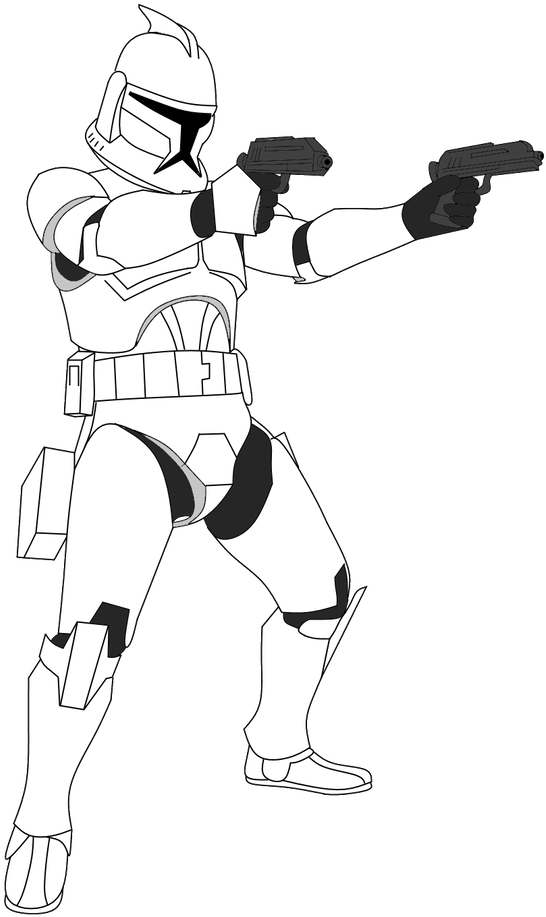
\includegraphics[width=0.3\textwidth]{continut/capitol4/figuri/clone_trooper.png}
    \caption{Clone Trooper\protect\footnotemark}
    \label{fig:clone_trooper}
\end{figure}
\footnotetext{imagine preluată de pe un site web care nu „merită” trecut la bibliografie \url{https://www.pngitem.com/}}

Tabelul \ref{tabel:tab_simplu} prezintă un exemplu foarte simplu de tabel în \LaTeX. Un alt exemplu este prezentat în Tabelul \ref{tabel:2} din \ref{anexa3:func_xyz}.

\begin{table}[ht]
    \centering
    \caption{Exemplu de tabel simplu}
    \label{tabel:tab_simplu}
    \begin{tabular}{||c l c r||} 
        \hline
        \textbf{Col1} & \textbf{Col2} & \textbf{Col3} & \textbf{Col4} \\
        \hline\hline
        1 & 6 & 87837 & 787 \\ 
        2 & 7 & 78 & 5415 \\
        3 & 545 & 778 & 7507 \\
        4 & 545 & 18744 & 7560 \\
        5 & 88 & 788 & 6344 \\
        \hline
    \end{tabular}
\end{table}

\subsection{Nivel 2}
\label{cap:cap4:nivel1:nivel2}

\subsubsection{Nivel 3}
\label{cap:cap4:nivel1:nivel2:nivel3}

\textcolor{gray}{\lipsum}

\textcolor{gray}{\lipsum}

\textcolor{gray}{\lipsum}

    \cleardoublepage

    \iffalse
\silentchapter{Concluzii}

Concluziile lucrării (1–2 pagini) în care se regăsesc cele mai importante concluzii din lucrare, care pornind de la obiectivele propuse în introducerea lucrării vor conține opinia personală a autorului privind rezultatele obținute în lucrare, o comparație a acestora cu alte proiecte/produse similare precum și posibile direcții de dezvoltare. 

\begin{itemize}
    \item Gradul în care s-a realizat tema propusă (motivarea eventualelor obiective modificate);
    \item Evidențierea concisă a contribuțiilor/soluțiilor personale (dacă este cazul);
    \item Comparație cu alte proiecte similare;
    \item Posibile direcții de dezvoltare.
\end{itemize}

În acest capitol nu se introduc figuri, table sau listing-uri de cod. Pot fi în schimb referite!

Concluziile finale au un rol semnificativ în cadrul lucrării de diplomă, care trebuie pus în evidență în special în momentul susținerii acesteia în fața comisiei. Aici trebuie prezentate, în câteva pagini, cele mai importante rezultate ale muncii depuse de candidat și potențiale direcții de dezvoltare ulterioară a temei abordate. Acest capitol oferă o sinteză a realizărilor obținute, precum și avantajele și neajunsurile soluțiilor alese. Concluziile nu trebuie să aducă rezultate sau interpretări noi, ci doar să le evidențieze pe cele din conținutul lucrării.

\section*{Direcții viitoare de dezvoltare}

\textcolor{gray}{\lipsum[1-3]}

\section*{Lecții învățate pe parcusul dezvoltării lucrării de diplomă}

\textcolor{gray}{\lipsum[2-4]}

\fi
    \cleardoublepage
    % *************** referinte bibliografice ***************
    \bibliographystyle{IEEEtran}
    \bibliography{bibliografie/bibliografie}
    \cleardoublepage
    
    % *************** anexe ***************
    %% config anexe
    %% refacem counter-ul de figuri/tabele/listing-uri, pentru a putea mentine
%% numerotarea si referirea corecta a figurilor din anexe
\setcounter{figure}{0}
\renewcommand{\thefigure}{A.\arabic{figure}}
\setcounter{table}{0}
\renewcommand{\thetable}{A.\arabic{table}}
%% reset counter capitole, sectiuni pentru anexe
\setcounter{chapter}{0}
\setcounter{section}{0}
\renewcommand{\thesection}{\arabic{section}}
%% titlul anexei in pagina
%% in cuprins va aparea doar numerotat
\titleformat
    {\section}
    [hang]
    {\color{albastru-ac}\bfseries\itshape}
    {Anexa \thesection.\ }
    {0pt}
    {}
    []
    \iffalse
\silentchapter{Anexe}
%% Nu se pot face referinte pe silentchapter => nu are sens sa pun label
% \label{cap:anexe}

Anexe prezintă doar elementele specifice proiectului!

Anexele (dacă este cazul) constituie o secțiune separată a lucrării care nu se numerotează ca și capitol. Anexele se numerotează crescător cu numere arabe (ex.: Anexa 1, Anexa 2 etc.). Anexele vor conține scheme, diagrame, secvențe din codul sursă.

\section{Componente Software}
\label{anexa1:comp_soft}

% \textit{Componente software:}
\begin{itemize}
    \item diagramele UML care referă numai la componentele dezvoltate de student și care datorită complexității pot fi listate pe o foaie de tip A3 sau A2.
    \item cod sursă numai pentru componentele dezvoltate de către student.
\end{itemize}

%% inserati \newpage inaintea fiecarui \section cu anexa pentru ca fiecare anexa sa inceapa pe pagina noua
\newpage
\section{Componente Hardware}
\label{anexa2:comp_hard}

% \textit{Componente Hardware:}
\begin{itemize}
    \item schemele electrice finale realizate într-un CAD de profil; 
    \item schemele cablajelor realizate pentru implementare, realizate într-un CAD de profil;
    \item informații suplimentare despre implementarea și testarea aplicației (de ex. capturi de osciloscop);
    \item schemele standard ce vor fi folosite pentru testare (pseudocod sau schemă logică);
    \item extrase din foi de catalog. 
\end{itemize}

%% inserati \newpage inaintea fiecarui \section cu anexa pentru ca fiecare anexa sa inceapa pe pagina noua
\newpage
\section{Codul funcției xyz()}
\label{anexa3:func_xyz}

În Figura \ref{fig:AT} este prezentat unul dintre cele mai impunătoare vechicule ale Imperiului.

\begin{figure}[H]
    \centering
    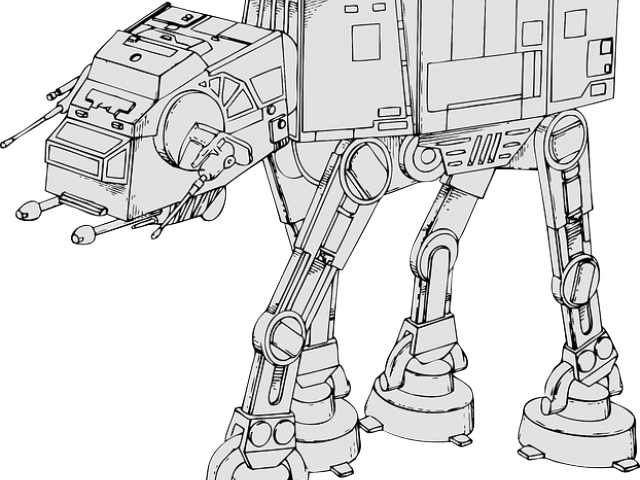
\includegraphics[width=0.5\textwidth]{anexe/figuri/AT.png}
    \caption{AT\protect\footnotemark}
    \label{fig:AT}
\end{figure}
\footnotetext{imagine preluată de pe un site web care nu „merită” trecut la bibliografie \url{https://www.pngitem.com/}}

\textcolor{gray}{\lipsum} (Figura \ref{fig:millennium_falcon})

\begin{figure}[H]
    \centering
    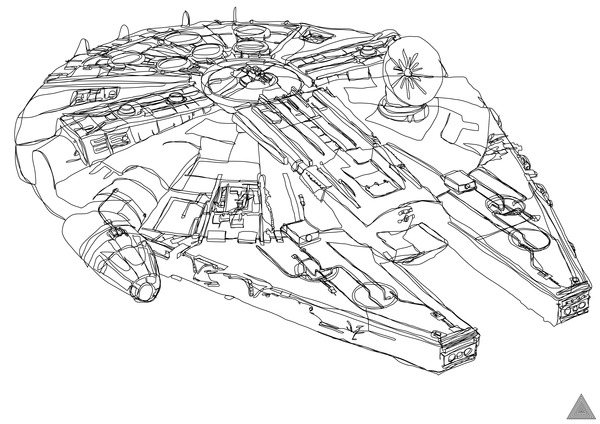
\includegraphics[width=0.8\textwidth]{anexe/figuri/millennium_falcon.jpeg}
    \caption{Millennium Falcon\protect\footnotemark}
    \label{fig:millennium_falcon}
\end{figure}
\footnotetext{imagine preluată de pe un site web care nu „merită” trecut la bibliografie \url{http://clipart-library.com/}}

%% inserati \newpage inaintea fiecarui \section cu anexa pentru ca fiecare anexa sa inceapa pe pagina noua
\newpage
\section{Tabel lung pe mai multe pagini}
\label{anexa4:long_table}

Malware (software rău intenționat) este un termen folosit pentru a descrie orice program sau cod care ocolește procesele de control al accesului, este creat cu intenția de a ataca un sistem de calcul sau rețea, pentru a provoca daune sau a compromite acel sistem. În categoria malware se includ: viruși, \textit{ransomware}, \textit{keyloggers}, troieni, viermi, \textit{spyware} etc (Tabelul \ref{tab_tipuri_de_malware}). În vocabularul curent, termenul de "virus" este folosit abuziv pentru orice tip de malware.

\begin{longtable}[c]{|l|p{6cm}|p{2cm}|}
	\caption{Tipuri de malware\label{tab_tipuri_de_malware}}\\
	
	\hline
	\multicolumn{1}{|c|}{\textbf{\textit{Tip}}} & 
	\multicolumn{1}{c}{\textbf{\textit{Descriere}}} & 
	\multicolumn{1}{|c|}{\textbf{\textit{Exemple elocvente}}}  \\
	\hline
	\endfirsthead
	
	\multicolumn{3}{c}{Continuarea tabelului \ref{tab_tipuri_de_malware}}\\
	\hline
	\multicolumn{1}{|c|}{\textbf{\textit{Tip}}} & 
	\multicolumn{1}{c}{\textbf{\textit{Descriere}}} & 
	\multicolumn{1}{|c|}{\textbf{\textit{Exemple elocvente}}}  \\
	\hline
	\endhead
	
	\hline
	\endfoot
	
	\hline
	\endlastfoot
	
	\multirow{8}*{Virus} &
	cod executabil malițios, atașat la fișiere sau programe legitime. Majoritatea virușilor necesită declanșarea de către utilizatorul final. Se răspândește prin intermediul unităților USB, discurilor optice, partajărilor în rețea sau e-mail-ului &
	%\multirow{6}*{Brain, Michelangelo, Melissa} \\  
	\newline \newline Brain, \newline Michelangelo, \newline Melissa \\
	\hline

	\multirow{5}{*}{Ransomware} & 
	conceput pentru a ține captiv un sistem informatic, de obicei prin criptarea datelor esențiale, dezactivează accesul victimei la date până la efectuarea unei plăți către atacator & 
	%\multirow{5}{*}{WannaCry, Petya} \\ 
	\newline WannaCry, \newline Petya \\	
	\hline
	
	\multirow{2}{*}{Fileless Malware} & 
	face modificări la fișierele native ale sistemului de operare & 
	\multirow{2}{*}{Astaroth} \\ 
	\hline
	
	\multirow{4}{*}{Spyware} & 
	proiectat pentru a urmări acțiunile utilizatorului și a colecta date despre activitatea victimei, fără cunoștința acesteia & 
	\multirow{4}{*}{DarkHotel} \\ 
	\hline
	
	\multirow{3}{*}{Adware} & 
	livrează anunțuri în mod automat. Unele sunt însoțite de programe \textit{spyware} & 
	\multirow{3}{*}{Fireball} \\ 
	\hline
	
	\multirow{5}{*}{Troian} & 
	execută operațiuni rău intenționate disimulate ca operațiuni dorite. Se deghizează în codul unui program cunoscut și se atașează de fișiere non-executabile & 
	\multirow{5}{*}{Emotet} \\ 
	\hline
	
	\multirow{7}{*}{Worms} & 
	se reproduce singur, se răspândește într-o rețea prin replicare, prin exploatarea vulnerabilităților din rețele. Au tipare similare, inclusiv o vulnerabilitate activă, o modalitate de a se propaga singuri și conțin un \textit{payload} & 
	\multirow{7}{*}{Stuxnet} \\ 
	\hline
	
	\multirow{9}{*}{Rootkit} & 
	conceput pentru a modifica sistemul de operare, astfel încât computerul să poată fi accesat de la distanță, printr-o portiță de acces. Rootkit-urile modifică privilegiile de acces, fișierele de sistem și instrumentele de monitorizare a sistemului, ceea ce le face foarte greu de detectat și eliminat & \multirow{9}{*}{Zacinlo} \\ 
	\hline
	
	\multirow{2}{*}{Keyloggers} & 
	monitorizează apăsările de taste ale victimei & 
	\multirow{2}{*}{Olympic Vision} \\ 
	\hline
	
	\multirow{3}{*}{Bots} & 
	lansează automat atacuri concertate si concentrate asupra sistemului țintă & 
	\multirow{3}{*}{Echobot} \\ 
	\hline
	
	\multirow{2}{*}{Mobile Malware} & 
	conțin cod specific (Android, iOS) infectării dispozitivele mobile & 
	\multirow{2}{*}{Triada} \\ 
	\hline	
\end{longtable}

%% inserati \newpage inaintea fiecarui \section cu anexa pentru ca fiecare anexa sa inceapa pe pagina noua
\newpage
\section{Tabel simplu}
\label{anexa5:simple_table}

Pentru a ușura lecturarea lucrării de diplomă recomandăm ca tabelele (dacă nu sunt prea mari) să nu fie împărțite (sparte) pe mai multe pagini.

\begin{table}[ht]
    \centering
    \caption{Rezultatele simulării}
    \begin{tabular}{|c|c|c|} 
        \hline
        \textbf{\textit{Tipul semnalului}} & \textbf{\textit{Durata}} & \textbf{\textit{Randamentul}} \\
        \hline
        sinusoidal & 10s & 99\% \\ 
        \hline
        dreptunghiular & 12s & 81\% \\
        \hline
        triunghiular & 15s & 89\% \\
        \hline
    \end{tabular}
    \label{tabel:2}
\end{table}

În Tabelul \ref{tabel:2} este prezentat un exemplu de formatare pentru un tabel cu cap de tabel orizontal.

%% inserati \newpage inaintea fiecarui \section cu anexa pentru ca fiecare anexa sa inceapa pe pagina noua
\newpage
\section{Cod în python}
\label{anexa6:listing_python}

\begin{code}
    \begin{minted}{python}
        import numpy as np
            
        def incmatrix(genl1,genl2):
            m = len(genl1)
            n = len(genl2)
            M = None #to become the incidence matrix
            VT = np.zeros((n*m,1), int)  #dummy variable
            
            #compute the bitwise xor matrix
            M1 = bitxormatrix(genl1)
            M2 = np.triu(bitxormatrix(genl2),1)
        
            for i in range(m-1):
                for j in range(i+1, m):
                    [r,c] = np.where(M2 == M1[i,j])
                    for k in range(len(r)):
                        VT[(i)*n + r[k]] = 1;
                        VT[(i)*n + c[k]] = 1;
                        VT[(j)*n + r[k]] = 1;
                        VT[(j)*n + c[k]] = 1;
                        
                        if M is None:
                            M = np.copy(VT)
                        else:
                            M = np.concatenate((M, VT), 1)
                        
                        VT = np.zeros((n*m,1), int)
            
            return M
    \end{minted} 
    \caption{Codul funcției \textit{incmatrix}} 
    \label{code:python_incmatrix}
\end{code}

%% inserati \newpage inaintea fiecarui \section cu anexa pentru ca fiecare anexa sa inceapa pe pagina noua
\newpage
\section{Cod în Kotlin (mai lung de o pagină)}
\label{anexa7:listing_kotlin}

\begin{code}
    \begin{minted}{kotlin}
internal inner class ScheduleAdapter : 
        RecyclerView.Adapter<CalendarSessionViewHolder>(),
        StickyHeaderHandler {
        
    private var schedule: MutableList<ScheduleItem> = mutableListOf()
    var data: List<SessionDataGroup> = emptyList()
        set(value) {
            updateSchedule(value)
            field = value
        }

    override fun onCreateViewHolder(
            parent: ViewGroup, 
            viewType: Int): CalendarSessionViewHolder {
        val view = when (viewType) {
            ScheduleItem.TYPE_SMALL ->
                    R.layout.item_schedule_session_header_small
            ScheduleItem.TYPE_LARGE -> 
                    R.layout.item_schedule_session_header_large
            else -> R.layout.item_schedule_session_card
        }

        val holder = layoutInflater.inflate(view, parent, false)
        return CalendarSessionViewHolder(holder, _favoriteNeedSync)
    }
    override fun getItemCount(): Int = schedule.size

    override fun onBindViewHolder(
        holder: CalendarSessionViewHolder, position: Int) {
        holder.show(schedule[position])
    }

    override fun getItemViewType(position: Int): Int {
        return schedule[position].type
    }
    private fun updateSchedule(groups: List<SessionDataGroup>) {
        val result = mutableListOf<ScheduleItem>()
        for (group in groups) {
            if (group.type == 0) {
                result += ScheduleItem.SmallHeader(
                    group.title, R.color.dark_grey_40
                )
                continue
            }
            if (group.type == 1) {
                result += ScheduleItem.LargeHeader(group)
                continue
            }

            result += ScheduleItem.LargeHeader(group)
            result += group.sessions.map { ScheduleItem.Card(it) }
        }

        schedule = result
    }
    override fun getAdapterData(): MutableList<*> = schedule
}
    \end{minted}
    \caption{clasa \textit{ScheduleAdapter}} 
    \label{code:kotlin_scheduleAdapter}
\end{code}

%% inserati \newpage inaintea fiecarui \section cu anexa pentru ca fiecare anexa sa inceapa pe pagina noua
\newpage
\section{Cod în XML (preluat din fisier)}
\label{anexa8:listing_xml}

\begin{code}
    \inputminted{xml}{anexe/coduri_sursa/pom.xml}
    \caption{Exemplu de cod XML preluat din fișier extern}
    \label{code:xml_pom}
\end{code}
\fi



    \cleardoublepage

\end{document}
